%   % !TEX root = ../../VIII,3_Rahmen-TeX_9-0.tex
%  
%   Band VIII, 3 N.~?? 	(Unter)rubrik Auszüge
%   Signatur/Tex-Datei:	LH_35_14_02_002,052.
%				
%   RK-Nr. 	58217
%				
%   Überschrift: 	(keine)
%   Titel: 			Aus und zu Borelli, De vi percussionis
%   Datierung:		Italien, März 1689-März 1690
%   LEd8-Wz803015, italienisches Papier
%
%   edlabels:			18
%   Diagramme: 		8
%
%
\selectlanguage{ngerman}
\frenchspacing
%
\begin{ledgroupsized}[r]{120mm}
\footnotesize
\pstart
\noindent\textbf{Überlieferung:}
\pend
\end{ledgroupsized}
%
\begin{ledgroupsized}[r]{114mm}
\footnotesize
\pstart \parindent -6mm
\makebox[6mm][l]{\textit{L}}%
Auszüge mit Bemerkungen aus 
\protect\index{Namensregister}{\textso{Borelli} (Borellus), Giovanni Alfonso 1608\textendash1679}\textsc{G.\,A.\,Borelli}, 
\cite{01001}\title{De vi percussionis}, Bologna 1667: 
LH~XXXV~14, 2~Bl.~2,~52. 
Ein Bogen~2\textsuperscript{o};
Wasserzeichen in Bl.~52 (italienisches Papier);
an den unteren Blattecken  geringfügiger Textverlust durch Papierschaden; 
untere Ecke von Bl.~2 abgerissen, Teilstück angeklebt.
Vier Seiten.
Für \lbrack\textit{Fig.~5}\rbrack, \lbrack\textit{Fig.~6}\rbrack\ und  \lbrack\textit{Fig.~7}\rbrack\ finden sich bei Borelli keine Vorlagen.
\pend
\end{ledgroupsized}
%
%
\vspace{5mm}
\begin{ledgroup}
\footnotesize
\pstart
\noindent%
\textbf{Datierungsgründe:}
Die Auszüge aus \protect\index{Namensregister}{\textso{Borelli} (Borellus), Giovanni Alfonso 1608\textendash1679}Borellis \cite{01001}\textit{De vi percussionis} von 1667
%
sind auf italienischem Papier verfasst und entstanden daher höchstwahrscheinlich während Leibnizens Aufenthalts in Italien (März 1689 bis März 1690).
%
\pend
%
\pstart
Nicht nur der Umfang und die Ausführlichkeit der Auszüge deuten darauf hin, dass Leibniz dort das Buch zum ersten Mal las; auch folgende Umstände lassen denselben Schluss zu.
%
Aus den zahlreichen Erwähnungen von 
%
\protect\index{Namensregister}{\textso{Borelli} (Borellus), Giovanni Alfonso 1608\textendash1679}Borelli  
%
in Leibnizens Schriften und Briefen vor 1689 geht keine direkte Kenntnis von \cite{01001}\textit{De vi percussionis} hervor. 
%
\protect\index{Namensregister}{\textso{Borelli} (Borellus), Giovanni Alfonso 1608\textendash1679}Borelli wird in erster Linie als großer Geometer und wegen seiner Version von
%
\protect\index{Namensregister}{\textso{Apollonios} von Perge um 260\textendash um 190 v. Chr.}Apollonius
%
angesprochen (z.\,B.\ \textit{LSB} III, 1, S.~376; III, 3, S.~38).
%
Selbst die Erwähnungen seiner naturphilosophischen Leistungen sind unspezifisch (z.\,B.\ \cite{00256}\textit{Hypothesis Physica Nova}, \textit{LSB} VI, 2, S.~254f.; \cite{01099}\textit{Brevis Demonstratio}, \textit{LSB} VI, 2, S.~2030)
%
oder beschränken sich auf seine bekannte These, dass die Stoßkraft unendlich sei (\textit{LSB} VIII, 2, S.~119, 162, 252; siehe \cite{01001}\textit{De vi percussionis}, Cap.~XXVII\textendash XXIX, S.~192\textendash210).
%
%
Aus einem \cite{02067}Schreiben
%
\protect\index{Namensregister}{\textso{Schuller}, Georg Hermann 1651\textendash1679}Schullers
%
für Leibniz vom April 1677 (\textit{LSB} III, 2, S.~78) ist bekannt, dass
%
\protect\index{Namensregister}{\textso{Tschirnhaus} (H.v.Tch., H.v.Tsch.), Ehrenfried Walther v. 1651\textendash1708}Tschirnhaus
%
bei \protect\index{Namensregister}{\textso{Regnauld} (Regnaud; Regnaldus), Fran\c{c}ois de 1626\textendash1689}F.~Regnauld in Lyon
%
verschiedene Werke \protect\index{Namensregister}{\textso{Borelli} (Borellus), Giovanni Alfonso 1608\textendash1679}Borellis, darunter \cite{01001}\textit{De vi percussionis} und \cite{02068}\textit{De motionibus naturalibus} von 1670, hatte einsehen können
%
\textendash\ Werke, die \protect\index{Namensregister}{\textso{Tschirnhaus} (H.v.Tch., H.v.Tsch.), Ehrenfried Walther v. 1651\textendash1708}Tschirnhaus
%
als \glqq scripta rariora\grqq\ bezeichnete.
%
In Italien bekam Leibniz zweifellos leichteren Zugang zu 
%
\protect\index{Namensregister}{\textso{Borelli} (Borellus), Giovanni Alfonso 1608\textendash1679}Borellis 
%
seltenen Büchern, als ihm in Hannover möglich gewesen war. %
\pend
%
\pstart
%
Obwohl wenige Jahre zuvor eine posthume Sammelausgabe beider obengenannten Abhandlungen 
%
erschienen war 
%
(\cite{02036}\textit{De vi percussionis, et motionibus naturalibus a gravitate pendentibus}, Leiden 1686), 
%
muss Leibniz die italienische Erstausgabe (Bologna 1667) verwendet haben:
%
Die einzige von ihm gemachte Seitenangabe 
%
(\glqq Et p.~49 addit\grqq, für die Passage auf S.~\refpassage{35_14_02_002,052_6a}{35_14_02_002,052_6b}) 
%
stimmt mit der \cite{01001}ersten Ausgabe
%
überein, nicht aber mit der \cite{02036}zweiten (die exzerpierte Stelle befindet sich auf S.~49 bzw.\ S.~37).
%
\pend
\end{ledgroup}
%
%
\selectlanguage{latin}
\frenchspacing
\newpage%
\count\Bfootins=1100%
\count\Afootins=1200%
\count\Cfootins=1100 
%\vspace{8mm}
\pstart%
\normalsize%
\noindent%
\lbrack2~r\textsuperscript{o}\rbrack\
%
%
\edtext{%	A-Fn
Borelli\protect\index{Namensregister}{\textso{Borelli} (Borellus), Giovanni Alfonso 1608\textendash1679} \textit{De percussione}}{\lemma{}\Afootnote{%
\textit{Am Rand}: %
\protect\index{Namensregister}{\textso{Borelli} (Borellus), Giovanni Alfonso 1608\textendash1679}Borelli 
liber ed.~2\textsuperscript{am} 1667\textsuperscript{\lbrack a\rbrack}
\newline\vspace{-0.5em}
\newline%Marginalienapparat:
{\footnotesize \textsuperscript{\lbrack a\rbrack} ed.~2\textsuperscript{am} 1667: Leibniz exzerpiert aus der \cite{01001}Erstausgabe, Bologna 1667; die \cite{02036}zweite Ausgabe erschien 1686.%
}}}
%
prop.~13.
%
\edtext{\textit{Si duo corpora aequalia inaequalibus velocitatibus moveantur eorum virtutes motivae eandem proportionem habebunt} 
\edtext{\textit{quam velocitates}.}{
\lemma{\textit{quam}}
\Bfootnote{\textit{(1)} velocitatem scilicet vim motivam in plano \textit{(2)} \textit{velocitates}. \textit{L}}}
%
Probatio intelligi nequit. Nempe vim motivam nihil
%
%
aliud esse quam nisum vel impetum, hic non potest percipi absque motione, itaque cum concipitur vis motiva dupla, seu duplus nisus concipitur agitatio dupla.}{%
\lemma{\textit{Si} \lbrack...\rbrack\ dupla}%
\Cfootnote{%
\protect\index{Namensregister}{\textso{Borelli} (Borellus), Giovanni Alfonso 1608\textendash1679}\textsc{G.\,A.\,Borelli}, \cite{01001}\title{De vi percussionis}, Bologna 1667, Prop.~XIII, S.~38f.}} %
\pend
%
\pstart
%
\edtext{Hinc prop.\
%
\edtext{\lbrack15.\rbrack}{%
\lemma{}%
\Bfootnote{%
14.
\textit{L ändert Hrsg.}}}
%
Si aequales vires motivae \textit{erunt velocitates reciproce proportionales corporibus}.}{%
\lemma{}%
\Cfootnote{\hspace{-2.45mm}Hinc \lbrack...\rbrack\ \textit{corporibus}: \cite{01001}a.a.O., Prop.~XV, S.~40.}}
%
\pend
%
\pstart
%
\edtext{\textls{Incidentia perpendicularis} est, quando linea perpendicularis ad corporis alterius superficiem, 
%
\textls{incidentia media} cum linea motus transit per centra gravitatis. Cum utrumque fit dicetur 
%
\textls{perpendicularis
%
\edlabel{35_14_02_002,052_1a}%
\edtext{}{{\xxref{35_14_02_002,052_1a}{35_14_02_002,052_1b}}{%
\lemma{\textls{et media.}}%
\Bfootnote{%
\textit{(1)} \textbar\ In \textit{streicht Hrsg.} \textbar\ medio cho \textit{(2)} Ex praef. \textit{L}} %
}}%
et media.}}{
\lemma{\textls{Incidentia} \lbrack...\rbrack\ \textls{media}}
\Cfootnote{a.a.O., Def.~I,
\cite{01001}S.~41.}} 
%
\pend  
%
\pstart  
%
Ex\edlabel{35_14_02_002,052_1b} praef.\
%
Borelli\protect\index{Namensregister}{\textso{Borelli} (Borellus), Giovanni Alfonso 1608\textendash1679}. 
\edtext{\textit{Galilaeus\protect\index{Namensregister}{\textso{Galilei} (Galilaeus, Galileus), Galileo 1564\textendash1642} 
%
in opusculo Mechanico edito juvenili aetate causam percussionis} inde assumsit, 
%
\textit{quod momentum potentiae} aequetur \textit{momento resistentiae}, quando \textit{reciproce velocitates proportionales} sunt \textit{potentiis scilicet} vastum corpus \textit{elevari ictu minoris}, 
%
quo \textit{ei communicatur velocitas quae ad velocitatem} percutientis sit ut \textit{potentia percutientis ad resistentiam percussi}, 
%
sed videt postea \textit{insufficientiam juvenilis ratiocinii}, et longe aliter se rem habere in percussione quam in trutina.}{%
\lemma{\textit{Galilaeus} \lbrack...\rbrack\ trutina}%
\Cfootnote{%
\cite{01001}a.a.O., Pro{\oe}mium, S.~\lbrack1f.\rbrack\ mit Auslassungen. %
}}
%
\pend
%
\pstart
%
\edtext{Ostendemus 
\edtext{inquit Borellus\protect\index{Namensregister}{\textso{Borelli} (Borellus), Giovanni Alfonso 1608\textendash1679}}{
\lemma{inquit Borellus}
\Bfootnote{\textit{erg. L}}}
%
%
potentiam percussivam esse ipsam molem corpoream.  
%
\textit{Malleus in actu percussionis}, etsi prius \textit{vehementissime} motus\lbrack,\rbrack\ \textit{non potest} moveri celerius quam \textit{corpus percussum}.}{%
\lemma{Os\hspace{0.1mm}}%
\Cfootnote{%
\hspace{-2.37mm}tendemus \lbrack...\rbrack\ \textit{percussum}: \cite{01001}a.a.O., S.~\lbrack3\rbrack\ mit Auslassungen.}}
%
\pend 
%
\pstart 
%
\hspace{1mm}\hspace{-1mm}% Trick, weil \edlabel nicht zu \par-Beginn sein darf
\edlabel{35_14_02_002,052_4a}%
\edtext{}{% C-Footnote 
{\xxref%
{35_14_02_002,052_4a}{35_14_02_002,052_4b}}%
\lemma{Mersennus \lbrack...\rbrack\ \textit{concludetur}}%
\Cfootnote{%
\cite{01001}a.a.O., \lbrack S.~4f.\rbrack\ mit Auslassungen.%
}}%
%
Mersennus\protect\index{Namensregister}{\textso{Mersenne} (Mersennus), Marin 1588\textendash1648} in Reflex.\
\edtext{$\phi$ys.~Math.\ cap.~23.\ communicavit}{
\lemma{$\phi$ys.~Math.}
\Bfootnote{\textit{(1)} publicavit \textit{(2)} cap.~23.\ communicavit \textit{L}}}
%
experimenta  
\edtext{Galilaei\protect\index{Namensregister}{\textso{Galilei} (Galilaeus, Galileus), Galileo 1564\textendash1642}}{
\lemma{Galilaei }
\Bfootnote{\textit{erg. L}}}
%{%\lemma{\textit{Mersennus} \lbrack...\rbrack\ [\textit{communicavit}]}%\Cfootnote{%\textsc{M. Mersenne}, \cite{00000}\title{Reflexiones Physico\textendash Mathematicae}, cap.~XXIII, S.~201\textendash203  in: Novae Observationes Physico\textendash Mathematicae, Paris 1647 (separate Paginierung).}} 
%
ipsi a Riccio\protect\index{Namensregister}{\textso{Ricci} (Riccius), Michelangelo 1619\textendash1682} % 
%
communicata. \textit{In medio chordae arcus annexo fune cubitali, cujus infimo termino pila plumbea 2 
unciarum pendebat, hanc demisit a summitate arcus notavitque flexionem ejus et tractionem chordae, deinde decem libras collocavit in medio chordae ejusdem arcus, quo detineretur chorda in eodem statu flexionis. Cum postea robustiorem arcum} sumsisset \textit{cujus chorda eodem pondere cadente ad minus spatium adduceretur}, notavit \textit{non posse detineri chordam a 10 libris in eo loco ad quem vi duarum unciarum cadentium} erat adducta, \textit{sed 20 libras requiri, unde concludebat arcum posse adeo robustum fieri,} 
%
\edtext{\textit{ut ne quidem}}{%
\lemma{\textit{ut}}%
\Bfootnote{%
\textit{(1)} nec %
\textit{(2)} \textit{ne quidem} %
\textit{L}%
}}
%
\textit{1000 librae possint illum in eo situ retinere}, %FN S. 3
in \textit{quem a 2 unciis ut antea cadentibus} erat \textit{adductus, qua propter vim percussionis aliqua ratione infinitam esse.} %
\pend
%
\pstart
\textit{Aliam observationem affert de globo plumbeo, quem attenuet malleus cadens ex unius brachii altitudine},  
\edtext{\textit{quam attenuationem licet prima vice}}{
\lemma{\textit{quam}}
\Bfootnote{\textit{(1)} altitudinem possit \textit{(2)} \textit{attenuationem licet} \textit{(a)} possit \textit{(b)} \textit{prima vice} \textit{L}}}
%
\textit{10 librae globum aequalem prementes} efficiunt\lbrack,\rbrack\ \textit{si} 
%
\edtext{\textit{tamen} \textit{ictu}}{%
\lemma{\textit{tamen}}%
\Bfootnote{%
\textit{(1)} ictus %
\textit{(2)} \textit{ictu} %
\textit{L}%
}}
%
\textit{repetito malleus suum globum plumbeum jam  
depressum ex eadem altitudine percutiat, novam depressionem faciet, quam non possint aliae librae, hoc est}  
\edtext{\textit{20 librae efficere}.}{
\lemma{}
\Bfootnote{\textit{20}
\textbar\ \textit{librae} \textit{erg.} \textbar\
\textit{efficere}.
\textit{L}}}
%
\textit{Quod si rursus idem urgeas, tandem vis percussionis infinita concludetur}.%
\edlabel{35_14_02_002,052_4b}
\pend
%
\pstart
%
\edtext{%
Et a \textit{fine dialogi 4ti de motu Galilaeus\protect\index{Namensregister}{\textso{Galilei} (Galilaeus, Galileus), Galileo 1564\textendash1642} 
innuit theoriam energiae percussionis esse perobscuram}, 
et \textit{ejus recessus remotos a primis} hominum \textit{imaginationibus}, et vim percussionis esse indeterminatam.
Promittebat alibi hoc demonstrare, sed nihil tale repertum.
Torricellius\protect\index{Namensregister}{\textso{Torricelli}, Evangelista 1608\textendash1647}  	
eadem prosecutus non demonstravit, sed conjecturis confirmavit vim percussionis esse infinitam.}{%
\lemma{Et a \textit{fine} \lbrack...\rbrack\ infinitam}%
\Cfootnote{\cite{01001}a.a.O., S.~\lbrack5f.\rbrack.}}
%
%
\edtext{\textit{Tandem post diuturnam} inquit Borellus\protect\index{Namensregister}{\textso{Borelli}, Giovanni Alfonso 1608\textendash1679} meditationem \textit{hanc}
%
\edtext{\textit{$\phi$ysicae Mathematicae partem}}{
\lemma{\textit{$\phi$ysicae}}
\Bfootnote{\textit{(1)} infinitam et \textit{(2)} \textit{Mathematicae partem} \textit{L}}}
%
\textit{puto me ex integro reperisse proprio marte.}
}{%
\lemma{\textit{Tandem} \lbrack...\rbrack\ \textit{marte}}%
\Cfootnote{%
\cite{01001}a.a.O., S.~\lbrack6\rbrack.}}
%
\pend  
%
\pstart  
\edtext{Si projectum ab aere impellitur a quo impelletur ipse aer.}{%
\lemma{\hspace{2mm}}%
\Cfootnote{%
 \hspace{-4.0mm}Si \lbrack...\rbrack\ aer: \cite{01001}a.a.O., Cap.~III, S.~10. %
}}
%
\pend  
%
\pstart
\edtext{Si fluidum careat condensabilitate, aequalis est  
\edtext{resistentia fluidi}{
\lemma{resistentia}
\Bfootnote{\textit{(1)} aeris \textit{(2)} fluidi \textit{L}}}
%
anterioris et conatus postici ad succedendum in ejus locum.}{%
\lemma{Si \lbrack...\rbrack\ locum}%
\Cfootnote{%
\cite{01001}a.a.O., Prop.~I, S.~12.}} 
%
\edtext{Sin fluidum sit condensabile est minor.}{%
\lemma{Sin \lbrack...\rbrack\ minor}%
\Cfootnote{%
\cite{01001}a.a.O., Prop.~II, S.~13.}}
%
\edtext{(\protect\vphantom)+ 
Saltem motus circa 
suum centrum non pendet a medii fluidi impulsu. 
Et ille tamen converti semper potest in alium. 
+\protect\vphantom()}{\lemma{}%
\Afootnote{\textit{Am Rand}: NB NB}}%
%
\pend  
\newpage
\count\Bfootins=1000%
\count\Afootins=1200%
\count\Cfootins=1000 
\pstart 
\edtext{Si duo corpora dura et inflexibilia\lbrack,\rbrack\ non potest \textit{A} totam suam velocitatem dare ipsi \textit{B}, nam quando \textit{B} ad eam velocitatem  
\edtext{pervenit quae}{
\lemma{pervenit}
\Bfootnote{\textit{(1)} \textbar\ ad \textit{streicht Hrsg.}\ \textbar\ quam \textit{(2)} quae \textit{L}}}
%
est ipsius \textit{A} residua, jam nullus amplius sit \edlabel{35_14_02_002,052_5a}impulsus.}{%
\lemma{Si \lbrack...\rbrack\ impulsus}%
\Cfootnote{%
\cite{01001}a.a.O., Prop.~XVIII, S.~43f. %
}}
%
\edtext{}{% 
{\xxref%
{35_14_02_002,052_5a}{35_14_02_002,052_5b}}%
\lemma{impulsus.}
\Bfootnote{\textit{(1)} (\protect\vphantom)+ Fingit quasi \textit{(2)} (+ Praesupponit successive transferri +) \textit{(3)} (\protect\vphantom)+ Loquitur \lbrack...\rbrack\ ratio \textit{(a)} nisi \textit{(b)} impulsus \lbrack...\rbrack\ impingens. +\protect\vphantom() \textit{(aa)} Si \textit{(bb)} Prop.~19 \textit{L}}}%
(\protect\vphantom)+ Loquitur quasi successive transferretur sed tamen non est ejus mens. +\protect\vphantom() 
(+ Ratio vera quod non est ratio impulsus nisi adeo ut corpus cel\textlangle eri\textrangle us, ergo non est ratio ut moveatur celerius quam ipsum impingens. +)
%
\pend  
%
\pstart 
Prop.~19.%
\edlabel{35_14_02_002,052_5b}
%
\edtext{\textit{Si corpus uniformiter latum, incidat in aliud corpus indifferens ad motum, hoc incidentis velocitatem retardabit, eritque} incidentis \textit{velocitas ad retardationem quam patitur ut summa} incidentium\lbrack,\rbrack\ corporis \textit{incidentis et percussi}\lbrack,\rbrack\ \textit{ad corpus percussum.}}{%
\lemma{\textit{Si} \lbrack...\rbrack\ \textit{percussum}}
\Cfootnote{
\cite{01001}a.a.O., Prop.~XIX, S.~46. % 
}}
%
\edtext{Supponit scilicet ambo postea moveri simul, contrarium fieri ex reflexione.}{%
\lemma{Supponit \lbrack...\rbrack\  reflexione}%
\Cfootnote{%
\cite{01001}a.a.O., Cor., S.~47.}}
%
\edlabel{35_14_02_002,052_6a}%	zwecks Referenzierung
Et p.~49 addit  
%
\edtext{\textit{quod tantopere aliqui peripatetici horrent videtur esse certissimum migrationem scilicet} 
%
\edtext{\lbrack\textit{mo}\rbrack\textit{tivae}}{%
\lemma{}%
\Bfootnote{%
activae %
\textit{L ändert Hrsg. nach Vorlage}%
}}
%
\textit{virtutis}.\edlabel{35_14_02_002,052_6b}}{
\lemma{\textit{quod} \lbrack...\rbrack\ \textit{virtutis}}
\Cfootnote{
\cite{01001}a.a.O., S.~49.}}  
%
\pend 
%		
\pstart 
\lbrack2~v\textsuperscript{o}\rbrack\ 
%
\edtext{Item ait ibidem initio  
%
%
\edtext{cap.~\lbrack7.\rbrack\ debere}{
\lemma{cap.}
\Bfootnote{\textbar\ 1.~\textit{ändert Hrsg.} \textbar\ \textit{(1)} posse \textit{(2)} debere \textit{L}}}
%
\textit{saltem prima corpora componentia hujus esse naturae}, ut sint \textit{omnino dura et inflexibilia}.}{%
\lemma{Item \lbrack...\rbrack\ \textit{inflexibilia}}%
\Cfootnote{%
\cite{01001}a.a.O., Cap.~VII, S.~49 mit Auslassungen.}}
%
\edtext{Gradus velocitatis amissae non reviviscit nisi a nova causa.}{%
\lemma{Gradus \lbrack...\rbrack\ causa}%
\Cfootnote{
\cite{01001}a.a.O., Supp.~II, S.~50f.}}
%
\pend  
%
\pstart 
\edtext{Corpus percussum uno instanti recipit totam velocitatem, 
%
\textit{oportet autem ambo esse omnino dura}.}{%
\lemma{Corpus \lbrack...\rbrack\ \textit{dura}}%
\Cfootnote{%
\cite{01001}a.a.O., Prop.~XX, S.~52.%
}}
%
\edtext{\textit{Impossibile est ut corpus dum vehitur impetu proprio destituatur} seu \textit{se habeat mere passive}. Videmus vehente quiescente ipsum porro continuare.}{%
\lemma{\textit{Impossibile} \lbrack...\rbrack\ continuare}%
\Cfootnote{%
\cite{01001}a.a.O., Prop.~XXII, S.~56.}}
%
\pend  
%
\pstart 
%
\edtext{\textit{Gassendus}\protect\index{Namensregister}{\textso{Gassendi} (Gassendus), Pierre 1592\textendash1655} 
%
\textit{cum de impressione impetus agit censet dum ab impellente} adhuc \textit{movetur} seu \textit{vehitur projectum assuescere} 
%
motui, quasi \textit{tirocinio} 
%
\edtext{\textit{quo}\lbrack\textit{d}\rbrack\textit{am}}{%
\lemma{}%
\Bfootnote{%
quoddam %
\textit{L ändert Hrsg.\ nach Vorlage}%
}}
%
\textit{unde fiat ut} postea \textit{per se} eum \textit{peragat}.}{%
\lemma{Gassendus \lbrack...\rbrack\ peragat}%
\Cfootnote{%
\cite{01001}a.a.O., Prop.~XXI, S.~55 mit Auslassungen.%
}}
%
\pend  
%
\pstart 
\edtext{%
\textit{Percussio} est \textit{actio compressiva}
%
\edtext{\textit{corporis} percu\lbrack ti\rbrack entis \textit{excepta}}{
\lemma{}
\Bfootnote{\textit{corporis} \textbar\ corporis \textit{streicht Hrsg.} \textbar\ percurrentis \textit{ändert Hrsg.} \textbar\ \textit{excepta} \textit{L}}}
\textit{a}
%
\edlabel{35_14_02_002,052_7a}%
\edtext{}{% B-Footnote – 
{\xxref%
{35_14_02_002,052_7a}{35_14_02_002,052_7b}}%
\lemma{percusso.}
\Bfootnote{\textit{(1)} \textit{Si corpora aequali velo} \textit{(2)}~Vires percussionum \textit{L}}}%
percusso.}{%
\lemma{\textit{Percussio} \lbrack...\rbrack\ percusso}%
\Cfootnote{%
\cite{01001}a.a.O., Cap.~X, S.~63.}}
%
\edtext{Vires percussionum%
\edlabel{35_14_02_002,052_7b}
%
in corpus non  
%
\edtext{amovibile quiescens\lbrack,\rbrack}{
\lemma{amovibile}
\Bfootnote{\textit{(1)} sunt \textit{(2)} quiescens \textit{L}}}
%
%
si omnia sint inflexibilia seu dura, sunt ut vires motrices seu  
%
Borello\protect\index{Namensregister}{\textso{Borelli} (Borellus), Giovanni Alfonso 1608\textendash1679}  
%
in composita ratione corporum et velocitatum.}{%
\lemma{Vires \lbrack...\rbrack\ velocitatum}%
\Cfootnote{%
\cite{01001}a.a.O., Prop.~XXVII, S~66.}}
%
\pend
\newpage
%%%%%%%%% Diagramm 1
\centerline{%
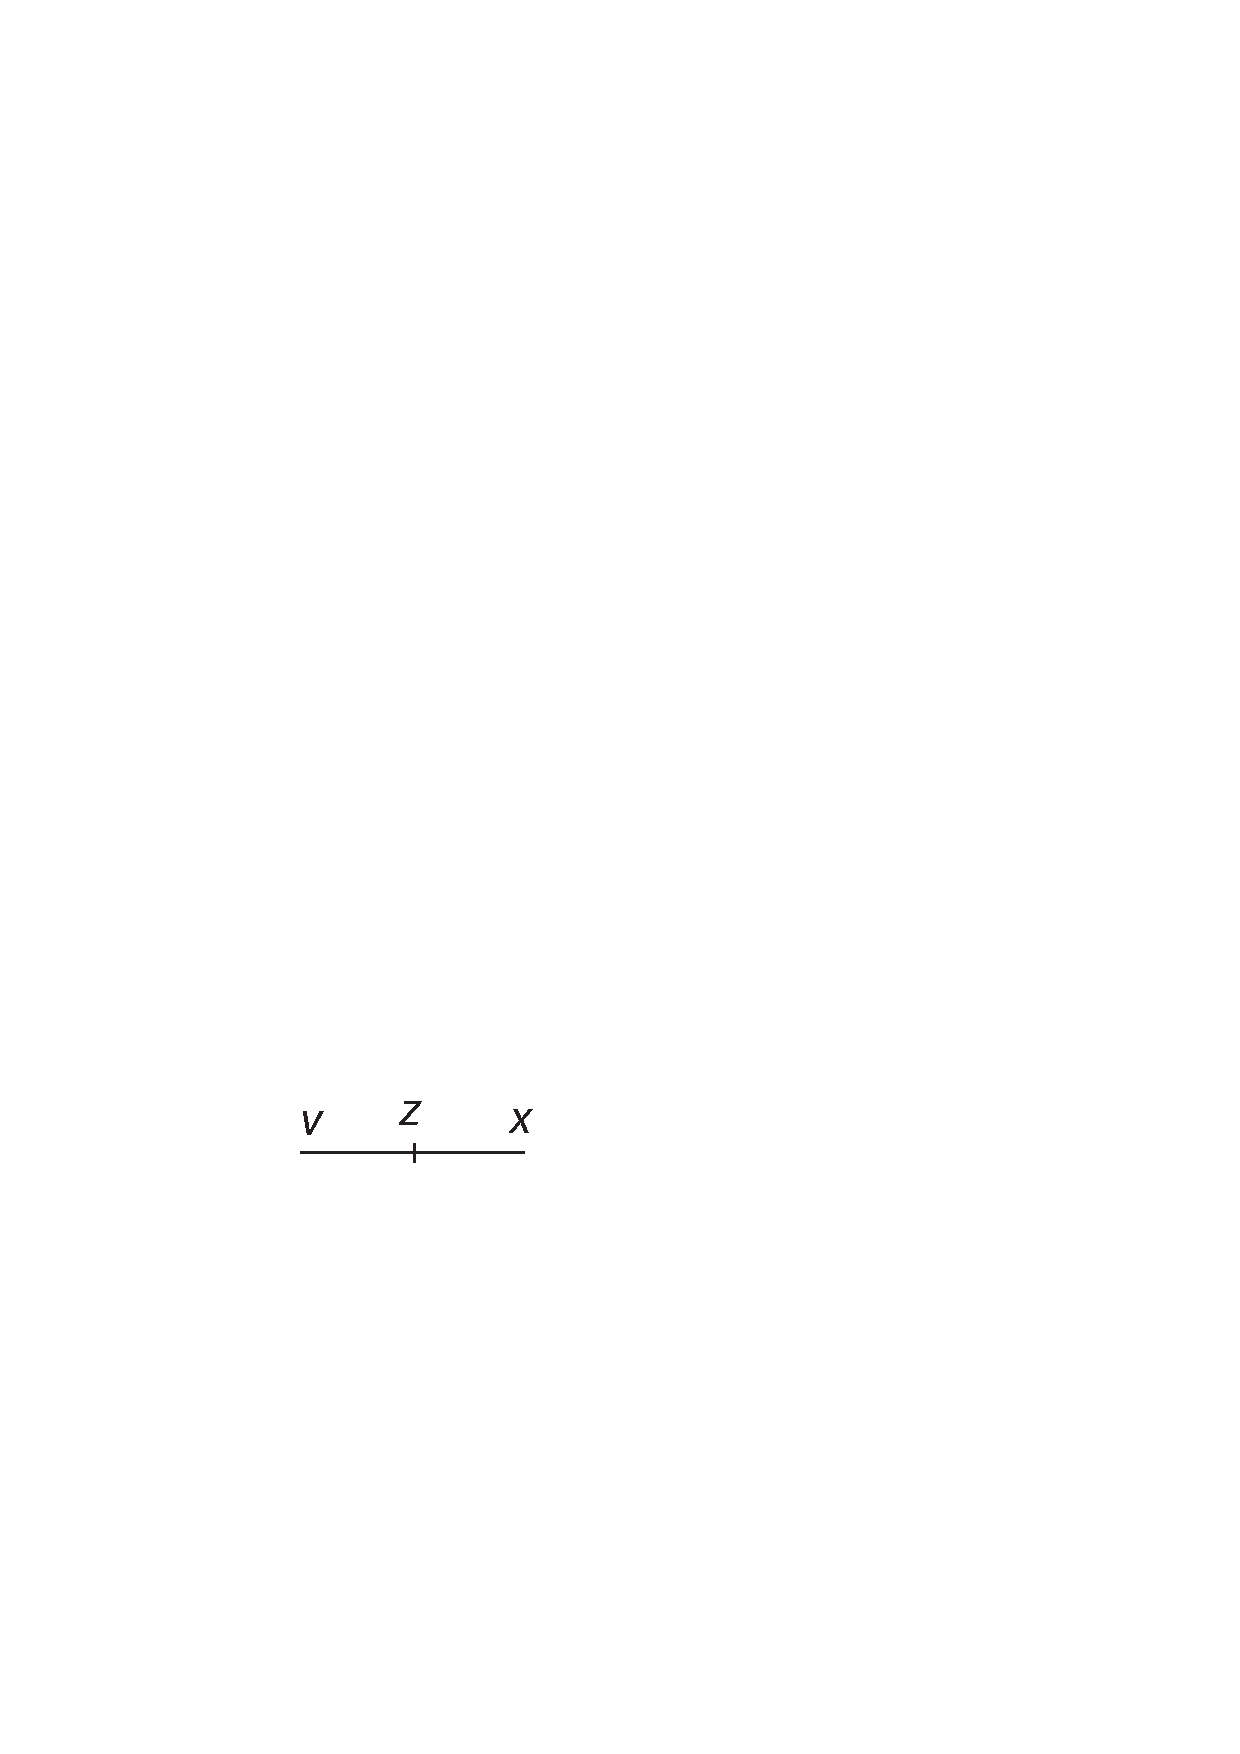
\includegraphics[width=0.15\textwidth]{%
gesamttex/edit_VIII,3/images/LH_35_14_02_002,052_d1_002r.pdf%
}} 
\vspace{0.5em}
\centerline{%
\lbrack\textit{Fig.~1}\rbrack%
}
% \newpage%
\vspace{1.0em}
%
\count\Bfootins=1100%
\count\Afootins=1200%
\count\Cfootins=1100 
\pstart
%
\edtext{\edlabel{35_14_02_002,052_8a}% Trick für Figur
}{\lemma{\hspace{1.8mm}\lbrack\textit{Fig.~1}\rbrack}\killnumber\Cfootnote{Tlw.\ Übernahme der Vorlage: \cite{01001}a.a.O., Tabula secunda, Fig.~25.}}%
%
\edtext{}{% C-Footnote 
{\xxref%
{35_14_02_002,052_8a}{35_14_02_002,052_8b}}%
\lemma{\textit{Vis} \lbrack...\rbrack\ celeritas}%
\Cfootnote{%
\cite{01001}a.a.O., Prop.~XXIX, S.~68f.}}%
%
\textit{Vis percussionis factae}
%
\edtext{a corpore \textit{A}}{
\lemma{}
\Bfootnote{a corpore \textit{A} \textit{erg. L}}}
%
\textit{super corpus}
%
\edtext{\textit{C}}{%
\lemma{}
\Bfootnote{\textit{C} \textit{erg. L}}}
%
%
\textit{quiescens} amovibile, \textit{mensuratur a portione impetus percussivi, ad quam}
%
\edtext{integra velocitas}{%
\lemma{integra velocitas}
\Bfootnote{\textit{erg. L}}}
%
\textit{eandem proportionem habet}
%
\textit{quam summa percutientis et percussi ad corpus percussum},
%
quae scilicet est retardatio ipsius corporis \textit{A}. 
%
Nempe \textit{A} habet 
%
velocitatem \textit{vx}\lbrack,\rbrack\ percussio
%
\edtext{erit}{%
\lemma{erit}
\Bfootnote{\textit{erg. L}}}
%
ut \textit{vz} quae ad \textit{vx} ut \textit{C} ad $A+C$. 
%
Nempe ipsi \textit{C} imprimitur velocitas \textit{xz}, qua non resistit ipsi \textit{A}, ergo resistit solum quatenus minor est haec celeritas.%
\edlabel{35_14_02_002,052_8b}
%
\pend 
%					
% 
\pstart 
%
\edtext{\textit{Si duo corpora dura et inflexibilia motibus contrariis per eandem rectam sibi mutuo occurrant, perpendiculari et media incidentia, percussio quae fieret super idem corpus tardius excurrens}\lbrack,\rbrack\ \textit{si in quiete amovibili} 
%
\edtext{\textit{constitu}\lbrack\textit{e}\rbrack\textit{retur}\lbrack,\rbrack}{
\lemma{constituretur}\Bfootnote{\textit{L ändert Hrsg. nach Vorlage}}} 
%
\textit{ad percussionem motibus contrariis factam eandem proportionem habet}\lbrack,\rbrack\ \textit{quam velocitas percutientis ad duas contrarias simul sumtas}.}{
\lemma{\textit{Si} \lbrack...\rbrack\  \textit{sumtas}}
\Cfootnote{\cite{01001}a.a.O., Prop.~XXXI, S.~71.}} 
%
\edtext{Ita prop.~31.}{
\lemma{}
\Bfootnote{Ita prop.~31. \textit{erg. L}}}		
%
\pend
%
\pstart
\hspace{1mm}\hspace{-1mm}% Trick, weil \edlabel nicht zu \par-Beginn sein darf
\edlabel{35_14_02_002,052_12a}%
\edtext{}{% C-Footnote 
{\xxref%
{35_14_02_002,052_12a}{35_14_02_002,052_12b}}%
\lemma{\textit{Si} \lbrack...\rbrack\ \textit{amo}\lbrack\textit{vi}\rbrack\textit{bili}}%
\Cfootnote{%
\cite{01001}a.a.O., Prop.~XXXII, S.~73.}}%
\textit{Si duo corpora contrariis motibus per eandem lineam rectam sibi occurrant perpendiculari et media incidentia} 
%
\edtext{\textit{impetus} (compressivus) \textit{quo}}{
\lemma{}
\Bfootnote{\textit{impetus} \textbar\ \textit{(1)}~compre \textit{(2)} (compressivus) \textit{erg.} \textbar\ \textit{quo} \textit{L}}}
%
\textit{unum ab} alio \textit{impellitur erit aequalis} 
%
\edtext{\textit{quo eorum}}{
\lemma{}
\Bfootnote{\textit{quo} \textbar\ eorum \textit{streicht Hrsg. nach Vorlage} \textbar\ \textit{eorum} \textit{L}}}
%
\textit{alterum velocitate aequali} duobus \textit{contrariis velocitatibus occurrit alteri quiescenti}
%
\edtext{\textit{amo}\lbrack\textit{vi}\rbrack\textit{bili}.\edlabel{35_14_02_002,052_12b}}{
\lemma{amobili}
\Bfootnote{\textit{L ändert Hrsg. nach Vorlage}}}
%
\edtext{Ita prop.~32.}{
\lemma{Ita prop.~32.}
\Bfootnote{\textit{erg. L}}}
%
In demonstratione addit: 
%
\edtext{impetus compressivus.}{
\lemma{impetus compressivus}
\Cfootnote{
\cite{01001}a.a.O., S.~73f.}}%
\pend
%
\pstart
%
\edtext{\textit{Si duo corpora ad easdem partes per eandem lineam moveantur et sibi mutuo occurrant}\lbrack,\rbrack\ \textit{impetus compressivus, quo corpus tardius fugiendo impellitur}\lbrack,\rbrack\ \textit{aequalis est impetui compressivo, facto in ejus quiete amovibili, velocitate differentiali}.}{
\lemma{\textit{Si} \lbrack...\rbrack\ \textit{differentiali}}
\Cfootnote{
\cite{01001}a.a.O., Prop.~XXXIII, S.~74.}} 
%
Prop.~33. 
%
\edtext{Demonstrationes propositionum 
%
\edtext{\lbrack32 et 33\rbrack}{%
\lemma{}%
\Bfootnote{%
31 et 32 %
\textit{L ändert Hrsg.}%
}}
%
parum satisfaciunt. 
%
Ex istis rursus demonstrat propositionem 31 in 
%
34.}{%
\lemma{Demonstrationes \lbrack...\rbrack\ 34}%
\Cfootnote{%
Die Prop.~32 und 33 werden als Prämissen eines zweiten, \glqq einfacheren\grqq\ (\textit{facilius}) Beweises der Prop.~31 eingeführt, den Borelli in Prop.~34 vollzieht; siehe die Bemerkungen \cite{01001}a.a.O., S.~73 und S.~75\textendash77.}}
%
Omnia ni fallor eo redeunt similiter ut ejus prop.~30.\ 31.\ vel 34. 
%
Ita habet propositionem 35\lbrack:\rbrack\ 
%
\edtext{si corpus alterum insequatur substituendam differentiam velocitatum.
%
Et in margine ponit: 
%
\textit{Energia percussionis non pendet ab impetu motus realis percutientis} 
%
\edtext{\textit{sed a motu}}{
\lemma{\textit{sed}}
\Bfootnote{\textit{(1)} ab impetu \textit{(2)} \textit{a motu} \textit{L}}}
%
\textit{respectivo}.}{%
\lemma{si corpus \lbrack...\rbrack\ \textit{respectivo}}%
\Cfootnote{%
\cite{01001}a.a.O., Prop.~XXXV, S.~77f.\ mit Auslassungen.}} 
%
\pend
\count\Bfootins=1100%
\count\Afootins=1100%
\count\Cfootins=1100 
%
\pstart
%		
\edtext{Si duo corpora concurrant lineis inter se angulum rectum facientibus, hinc perinde est ac si corpus excipiens quiesceret.}{%
\lemma{Si \lbrack...\rbrack\ quiesceret}%
\Cfootnote{%
\cite{01001}a.a.O., Prop.~XXXVI, S.~78f.}}
%
\pend
%
\vspace{1.0em} %%%%%%%%% Diagramm 2
\centerline{%
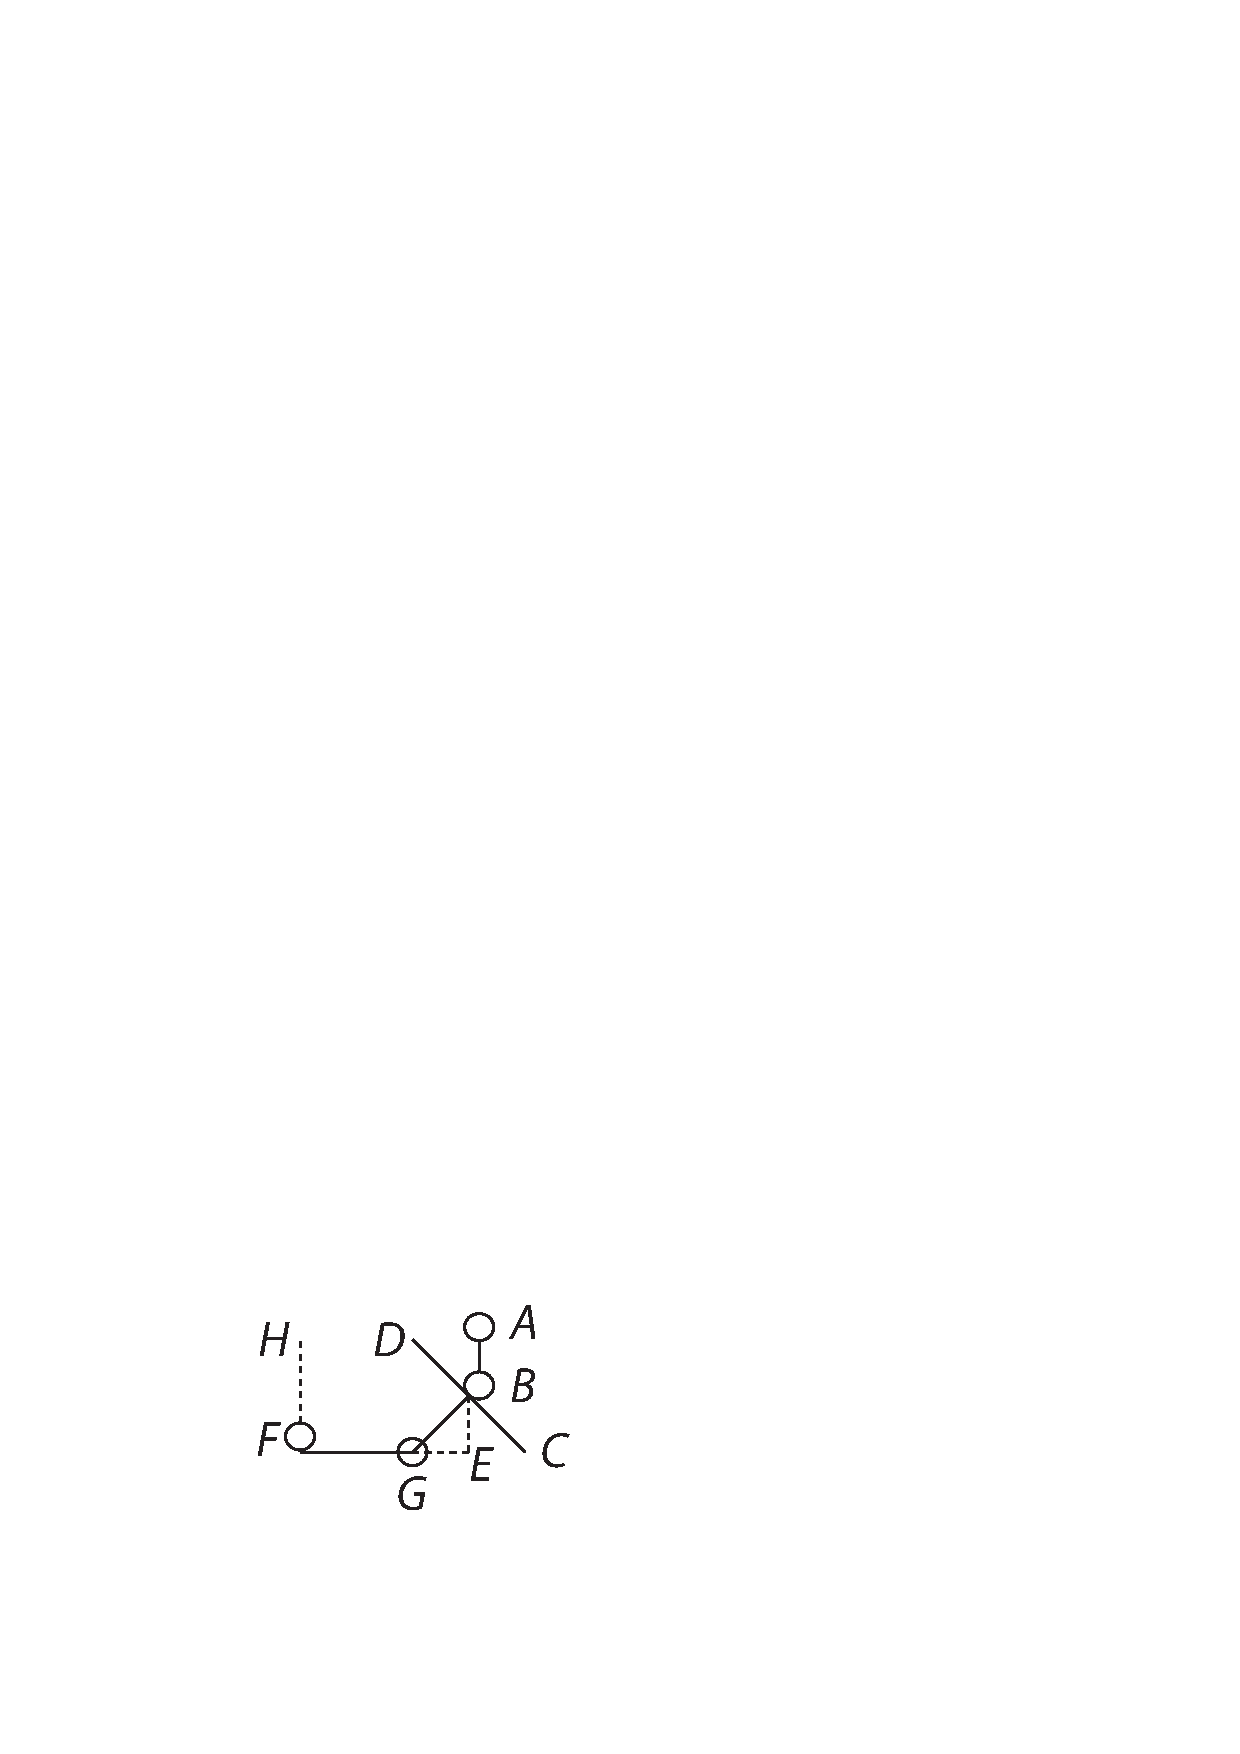
\includegraphics[width=0.2\textwidth]{%
gesamttex/edit_VIII,3/images/LH_35_14_02_002,052_d2_002r.pdf%
}} 
\vspace{0.4em}
\centerline{%
\lbrack\textit{Fig.~2}\rbrack%
}
%
\vspace{1.0em}
%
\pstart
%
\edtext{\edlabel{35_14_02_002,052_18a}}{% Trick für Zeichnung
\lemma{\lbrack\textit{Fig.~2}\rbrack}\killnumber\Cfootnote{\cite{01001}Tlw. Übernahme der Vorlage: a.a.O., Tabula secunda, Fig.~34.}}%
\edtext{}{% C-Footnote
{\xxref%
{35_14_02_002,052_18a}{35_14_02_002,052_18b}}%
\lemma{Si \lbrack...\rbrack\ ad \textit{GE}}%
\Cfootnote{%
\cite{01001}a.a.O., Prop.~XXXX, S.~83f.}}%
%
Si corpus \textit{B} linea \textit{AB} impingat in planum inclinatum \textit{CD}, perinde est %
%
\edtext{Borello\protect\index{Namensregister}{\textso{Borelli} (Borellus), Giovanni Alfonso 1608\textendash1679}, ad}{%
\lemma{Borello,}%
\Bfootnote{%
\textit{(1)} ac si %
\textit{(2)} ad  %
\textit{L}%
}}
%
impressionem perpendicularem, ut est vis ipsius \textit{F} incurrentis linea 
%
\edtext{\textit{HF}, in}{
\lemma{\textit{HF},}
\Bfootnote{\textit{(1)} ad \textit{(2)} in \textit{L}}}
%
brachium librae obliquae \textit{FGB} mobilis circa \textit{B}, ad vim ipsius \textit{B} incurrentis linea \textit{AB}, ubi constat esse 
%
\edtext{momenta \textit{F}}{\lemma{momenta}\Bfootnote{\textit{(1)} ut \textit{FE} \textit{(2)} \textit{F} \textit{L}}}
%
et \textit{B}, ut \textit{FG}
%
\edlabel{35_14_02_002,052_2a}%
\edtext{}{{\xxref{35_14_02_002,052_2a}{35_14_02_002,052_2b}}%
\lemma{ad \textit{GE}.}%
\Bfootnote{\textit{(1)} Motus corporis \textit{(2)} Motum \textit{AB} \textit{L}}}%
%
ad \textit{GE}.%
\edlabel{35_14_02_002,052_18b} 
%
\pend 
%
\vspace{1.0em} %%%%%%%%% Diagramm 3
\centerline{%
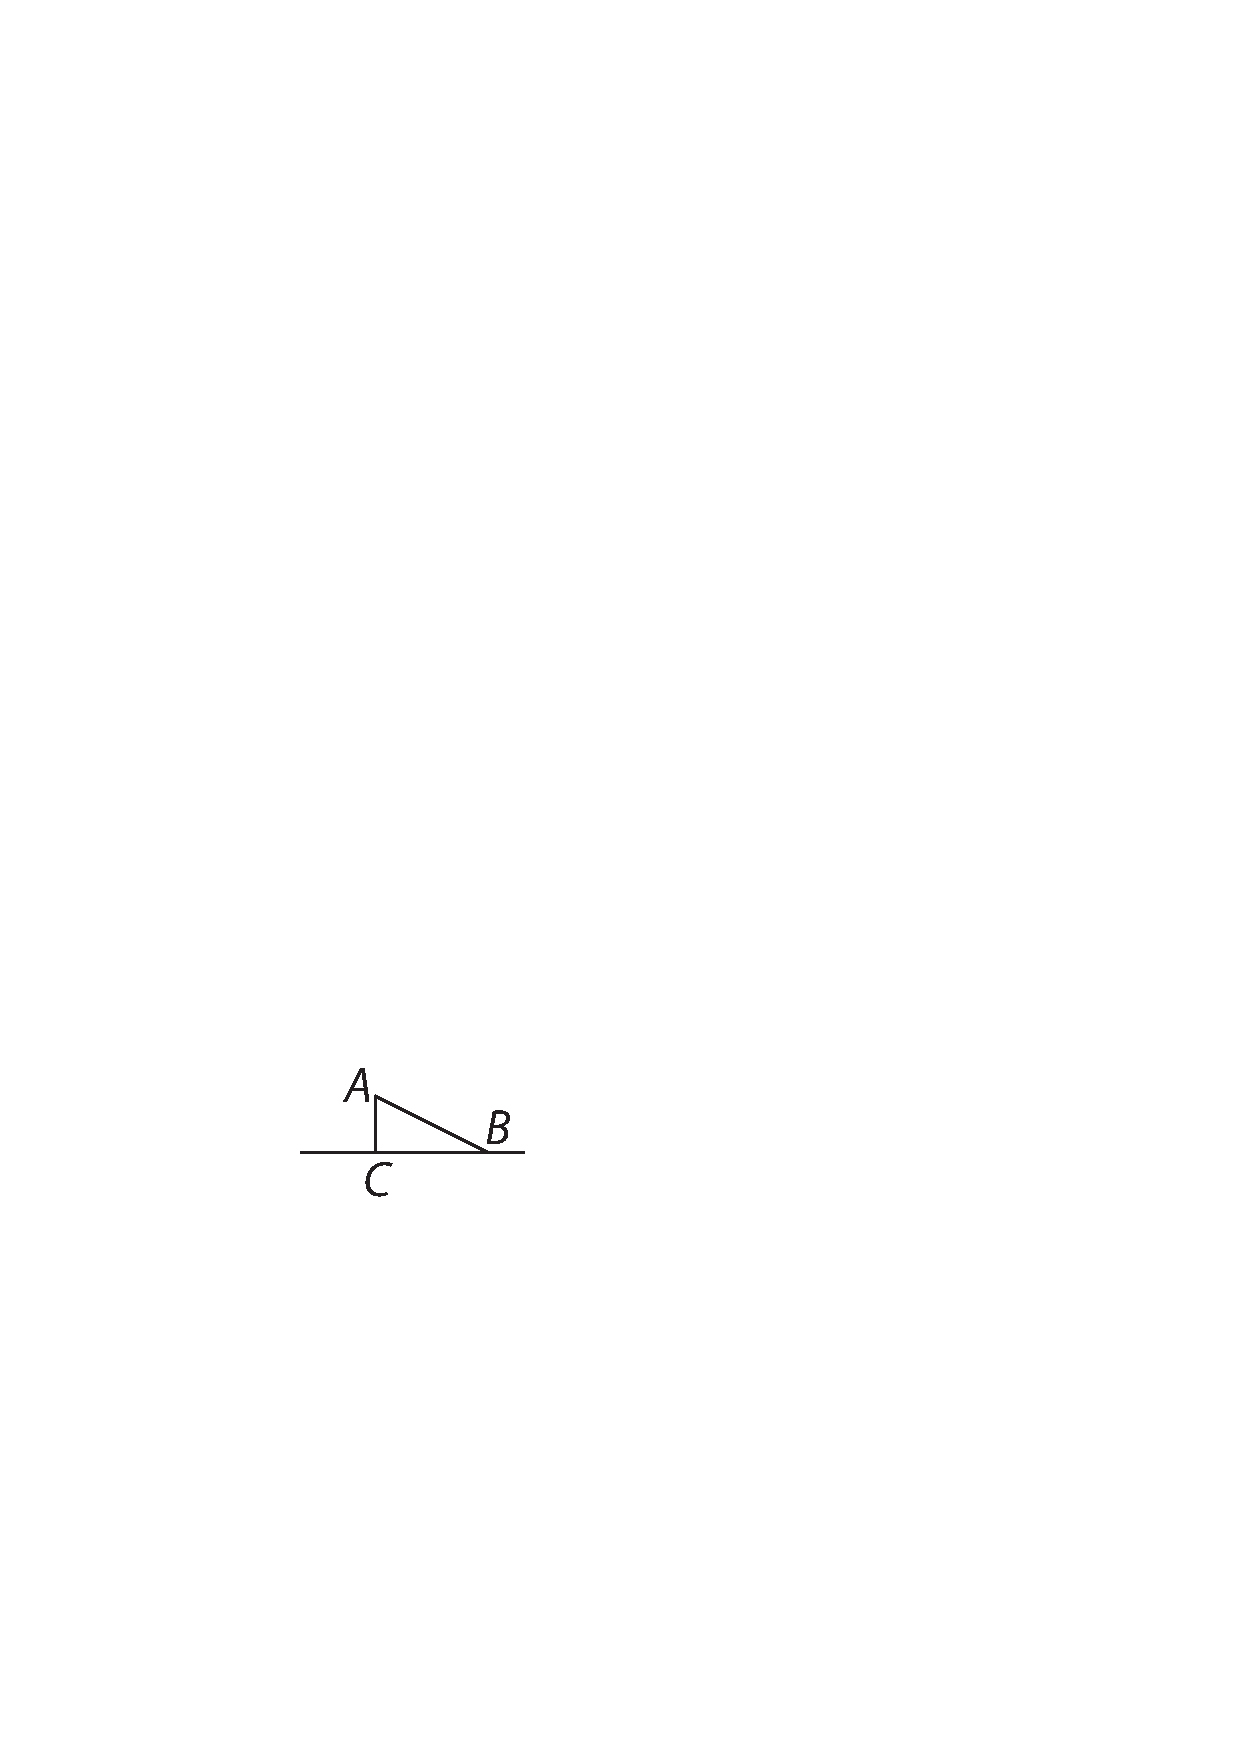
\includegraphics[width=0.15\textwidth]{%
gesamttex/edit_VIII,3/images/LH_35_14_02_002,052_d3_002r.pdf%
}} 
\vspace{0.4em}
\centerline{%
\lbrack\textit{Fig.~3}\rbrack%
}
% \newpage%
\vspace{1.0em}
%
\pstart 
%
\edtext{\edlabel{35_14_02_002,052_14a}}{%	% Trick für Figur
\lemma{\hspace*{1,6mm}%
\lbrack\textit{Fig.~3}\rbrack%
}\killnumber%
\Cfootnote{%
Tlw.\ Übernahme der Vorlage: a.a.O., Tabula secunda, Fig.~38.}}%
%
\edtext{}{% C-Footnote
{\xxref%
{35_14_02_002,052_14a}{35_14_02_002,052_14b}}%
\lemma{Motum \lbrack...\rbrack\ \textit{BC}}%
\Cfootnote{%
\cite{01001}a.a.O., Prop.~XXXXV, S.~90.%
}}%
Motum \textit{AB}\edlabel{35_14_02_002,052_2b} componit ex \textit{AC} et \textit{BC}.%
\edlabel{35_14_02_002,052_14b}
%
\pend
%
\pstart
Ex istis infert 
%
\edtext{prop.~\lbrack46.\rbrack}{%
\lemma{}%
\Bfootnote{%
36. %
\textit{L ändert Hrsg.}}}
%
\edtext{quam ait primo aspectu esse incredibilem et paradoxam:}{%
\lemma{quam ait \lbrack...\rbrack\ paradoxam}%
\Cfootnote{%
\cite{01001}a.a.O., S.~91.\hspace{-3mm}}}
%
\edlabel{35_14_02_002,052_9a}%
\edtext{}{% C-Footnote 
{\xxref%
{35_14_02_002,052_9a}{35_14_02_002,052_9b}}%
\lemma{\textit{si} \lbrack...\rbrack\ \textit{erunt}}%
\Cfootnote{%
\cite{01001}a.a.O., Prop.~XXXXVI, S.~91.%
}}%
\edtext{}{{\xxref{KZeitz203}{KZeitz204}}%
{\lemma{}\Afootnote{\textit{Am Rand}: elegans\vspace{-4mm}}}}%
\edlabel{KZeitz203}\textit{si duo corpora aequalia et similaria aeque disteterint a plano subjecto omnino stabili atque}
\pend
\newpage
\pstart
\noindent \textit{motu aequabili eodem tempore}
%
\textit{ad contactum plani subjecti perveniant}\lbrack,\rbrack\ \textit{unum quidem perpendiculari transitu}\lbrack,\rbrack\ \textit{alterum}
%
\edtext{\textit{ad}}{
\lemma{}
\Bfootnote{\textit{ad} \textit{erg. L}}}
%
\textit{idem planum inclinato}\lbrack,\rbrack\ 
%
\textit{eorum vires et energiae percussionum aequales erunt.}%
\edlabel{35_14_02_002,052_9b}\edlabel{KZeitz204}
%
\edtext{\lbrack52~r\textsuperscript{o}\rbrack}{%	% Trick für Figur
\lemma{\hspace*{1,6mm}%
\lbrack\textit{Fig.~4}\rbrack%
}\killnumber%
\Cfootnote{%
Tlw.\ Übernahme der Vorlage: a.a.O., Tabula secunda, Fig.~40.}}
%
\pend
%
%
\vspace{1.0em} %%%%%%%%% Diagramm 4
\centerline{%
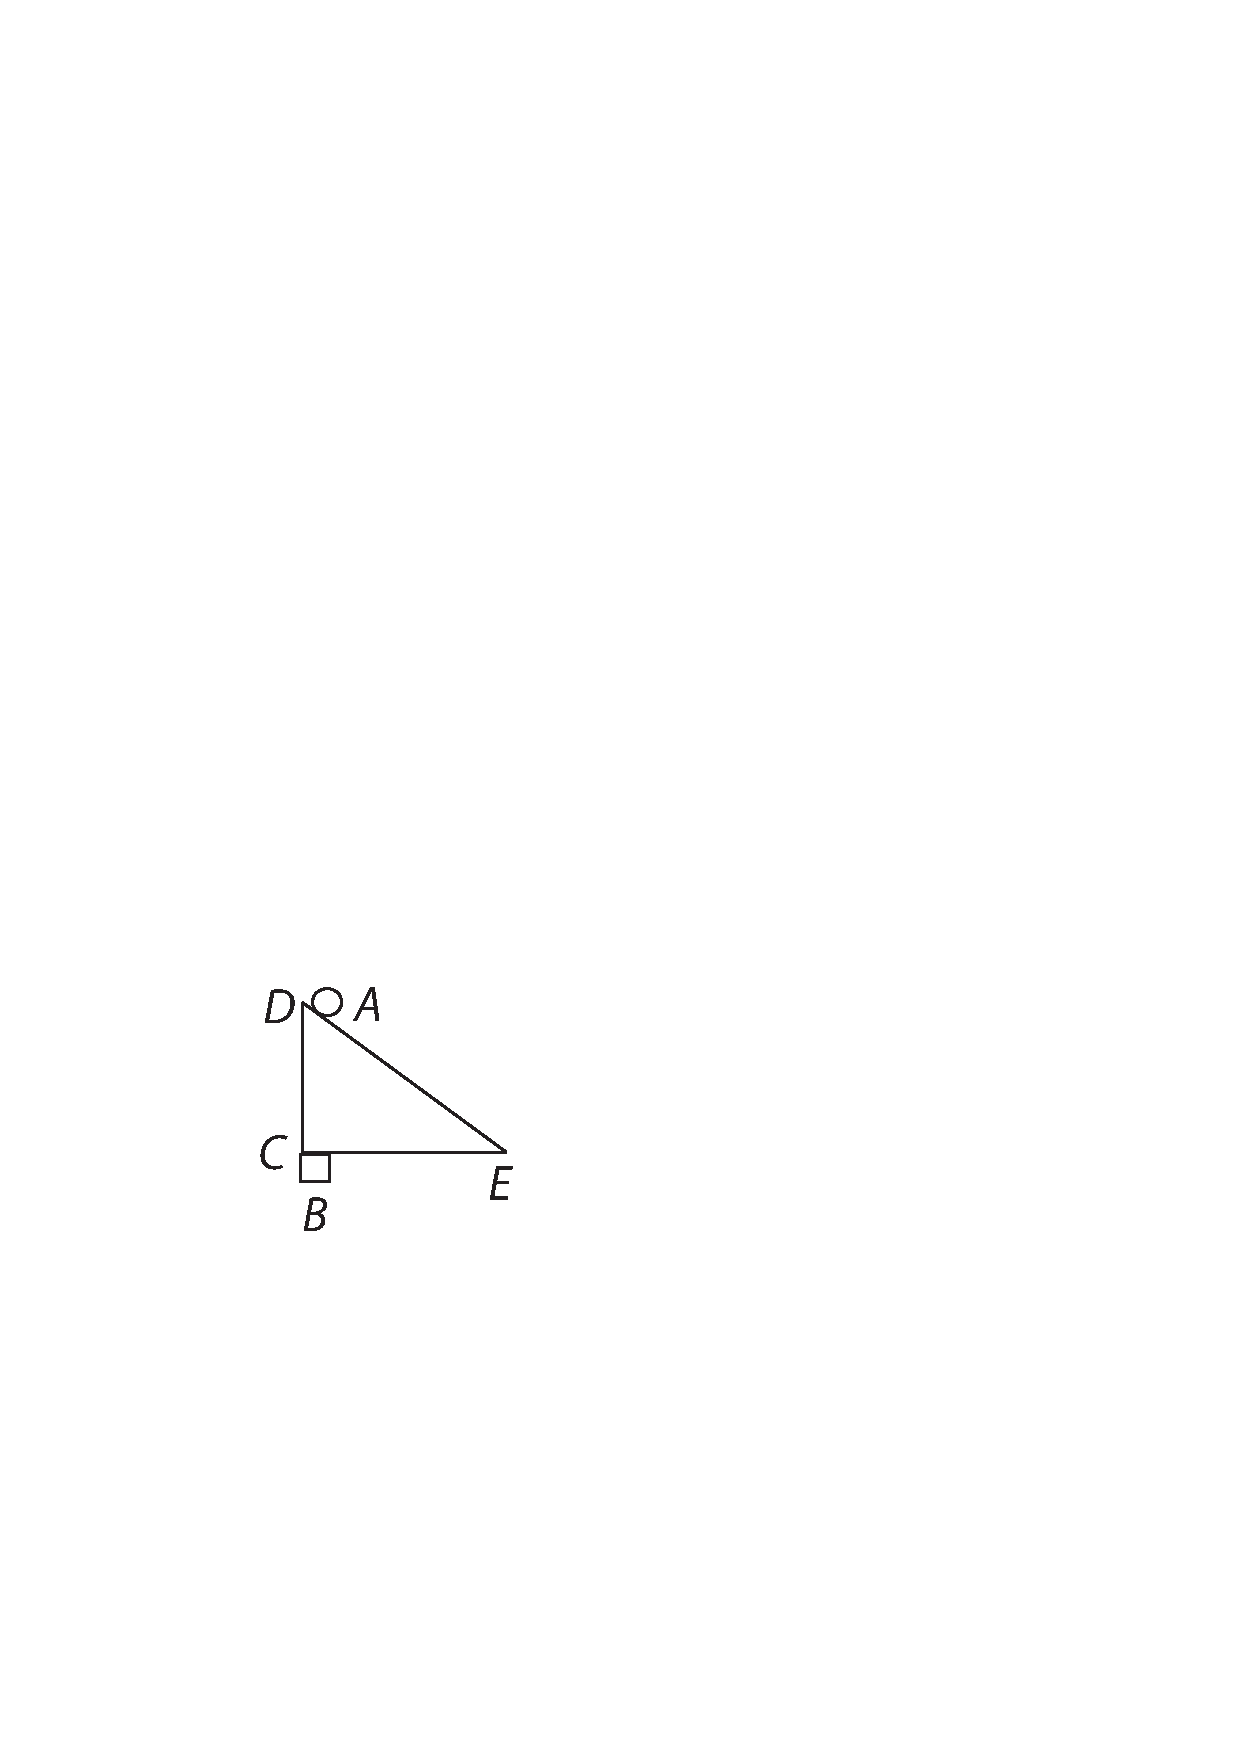
\includegraphics[width=0.175\textwidth]{%
gesamttex/edit_VIII,3/images/LH_35_14_02_002,052_d4_052r.pdf%
}} 
\vspace{0.5em}
\centerline{%
\lbrack\textit{Fig.~4}\rbrack}
% \newpage%
\vspace{1.0em}
%
%
\pstart 
%
\edtext{%
Si moveatur \textit{B} per \textit{CE} et \textit{A} per \textit{DE} perinde occurrent 
%
\edtext{sibi in \textit{E}}{%
\lemma{sibi}%
\Bfootnote{%
\textit{(1)} ac %
\textit{(2)} in \textit{E} %
\textit{L}%
}}
%
ac 
%
\edtext{si \textit{A} \textit{B} quiescenti occurreret}{
\lemma{si \textit{A}}
\Bfootnote{\textit{(1)} ei \textit{(a)} occurret \textit{(b)} occurreret \textit{B} \textit{(2)} \textit{B} quiescenti occurreret \textit{L}}}
%
in \textit{CD}, potest enim intelligi ferri \textit{A} 
%
\edtext{motu transversali ipsius \textit{CD} per \textit{CE},}{
\lemma{motu}
\Bfootnote{\textit{(1)} simpli \textit{(2)} transversali \textit{(a)} per  \textit{(aa)} \textit{CD} ipsi \textit{(bb)} \textit{CE} \textit{(b)} ipsius \textit{CD} per \textit{CE}, \textit{L}}}
%
et simul motu descensus per \textit{CD}, et solus descensus per \textit{CD} impetum faciet in \textit{B} motum motu solo ipsius \textit{DC}.}{%
\lemma{Si \lbrack...\rbrack\ ipsius \textit{DC}}%
\Cfootnote{%
\cite{01001}a.a.O., Prop.~XXXXVIII, S.~94f.}}
%
\pend
%
\pstart
%
\edtext{%
\textit{Si fuerint corpora tria} (+ plura \lbrack+\rbrack) \textit{aequalia mole}\lbrack,\rbrack\ \textit{figura}\lbrack,\rbrack\ \textit{positione, consistentia, et duritie}\lbrack,\rbrack\ \textit{aeque remota a plano subjecto, 
%
quorum} alterum \textit{simplici motu perpendiculari ad planum subjectum moveatur, duo vero reliqua motu obliquo, sed omnia 
%
motu aequabili ferantur, ita ut unum postremorum oblique incidat super planum subjectum stabile et firmum}\lbrack,\rbrack\ \textit{reliquum vero 
%
incidat super planum id ipsum subjectum sed agitatum}\lbrack,\rbrack\ \textit{sive ad easdem partes sive non, erunt praedictae tres percussiones 
%
ejusdem prorsus energiae}\lbrack,\rbrack\ quia \textit{omnes mensurantur ab impetu perpendiculari qui est idem.}}{%
\lemma{\textit{Si} \lbrack...\rbrack\ \textit{idem}}%
\Cfootnote{%
a.a.O., Prop.~XXXXX, S.~100.}}%
\pend
%
\pstart
%
\edtext{Si murus machina bellica ex 
%
eodem loco pila amissa percutiatur\lbrack,\rbrack\ semper erit eadem vis sive directe sive 
%
oblique\lbrack,\rbrack\ mensurabitur enim a perpendiculari distantia. \textit{Oportet} tamen \textit{ut planum subjectum} 
%
\edtext{\textit{sit durum},}{%
\lemma{}%
\Bfootnote{%
\textit{sit} \textbar\ satis \textit{gestr.}\ \textbar\ %
\textit{durum}, \textit{L}}}
%
ne aliquid abradatur. 
%
Nam per abrasionem 
%
\edtext{mutatur superfi\lbrack ci\rbrack es.}{%
\lemma{}%
\Bfootnote{%
mutatur \textbar\ plani \textit{gestr.}  \textbar\ superficies \textit{ändert Hrsg.} \textbar\ . \textit{L}}}%
}{% C-Fn
\lemma{\hspace{1.8mm}}%
\Cfootnote{%
\hspace{-4.0mm}Si \lbrack...\rbrack\ superfi\lbrack ci\rbrack es: \cite{01001}a.a.O., Prop.~LV, S.~106.}}
%
\pend 
\newpage
\centerline{%
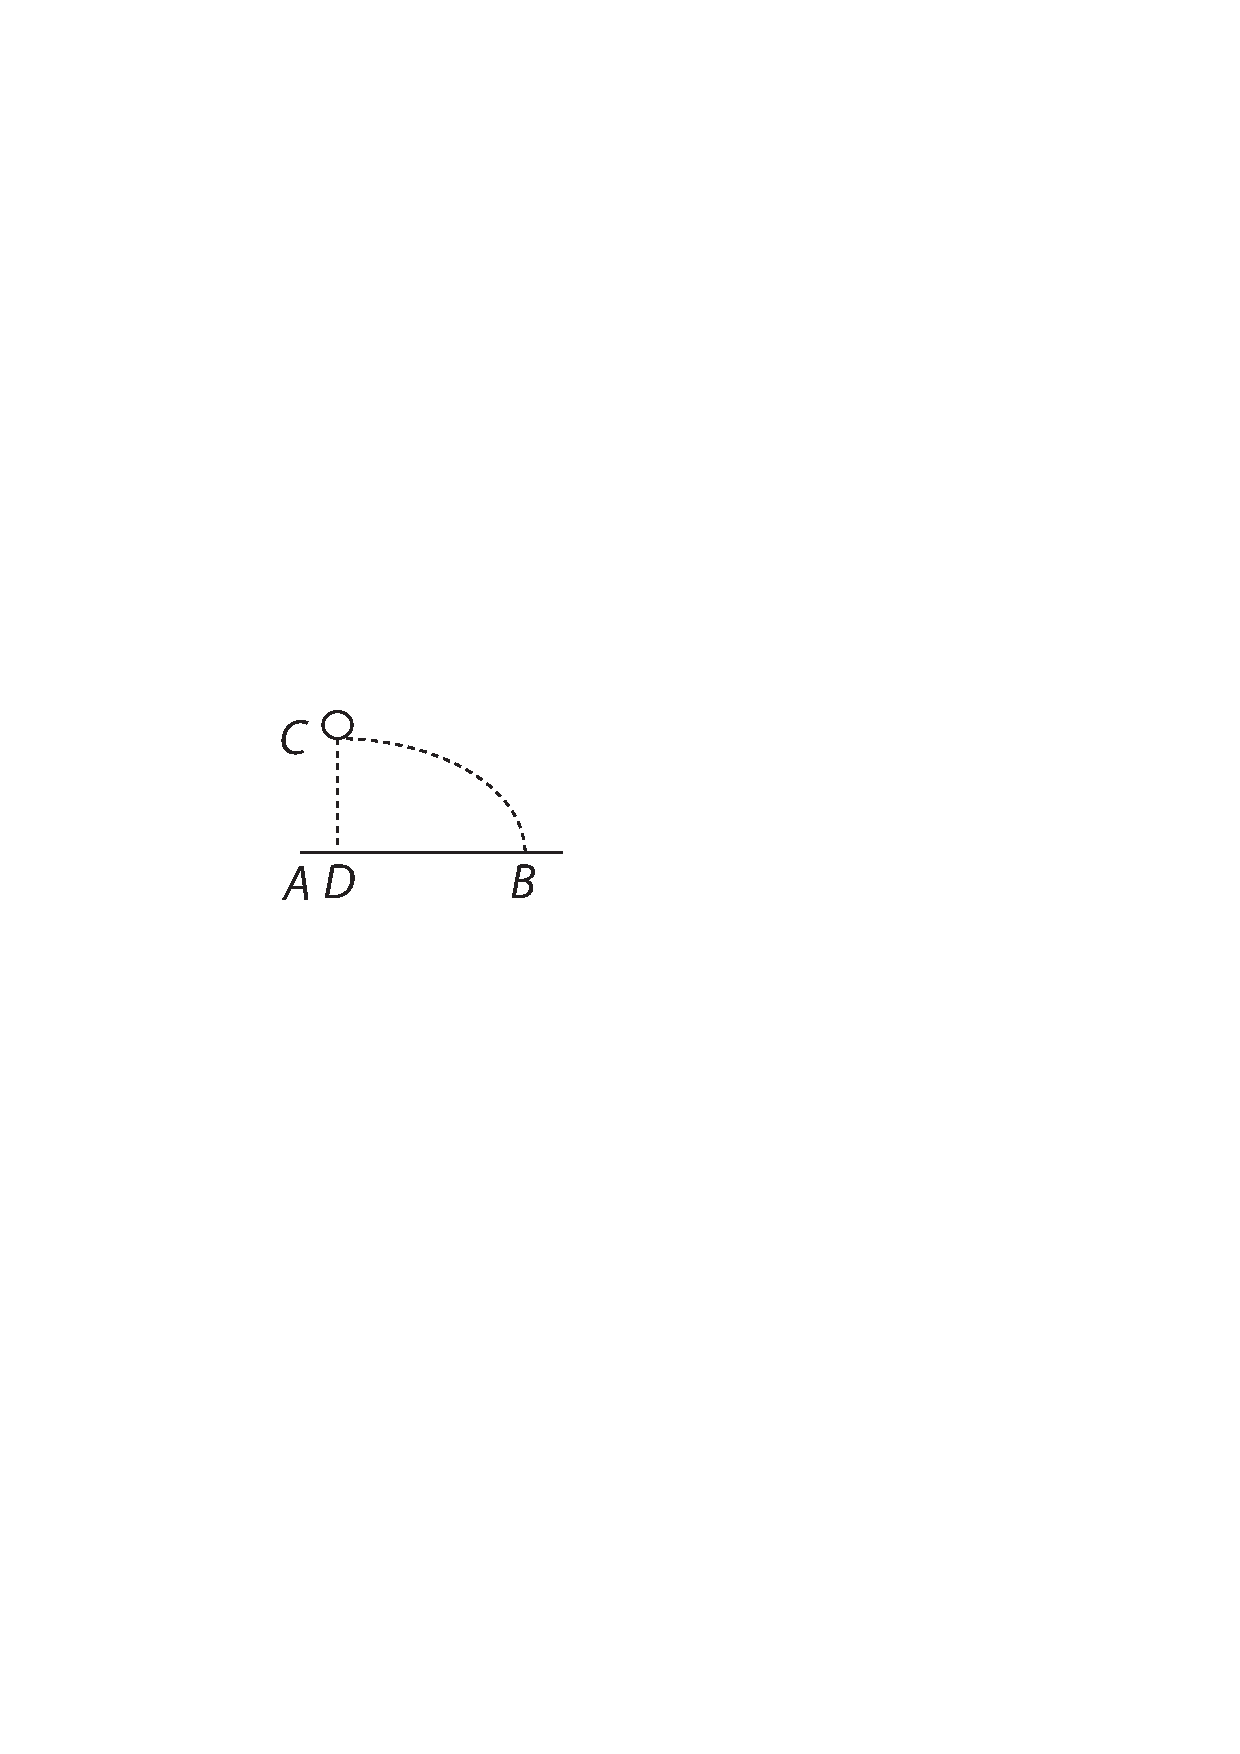
\includegraphics[width=0.18\textwidth]{%
gesamttex/edit_VIII,3/images/LH_35_14_02_002,052_d5_052r.pdf%
}} 
\vspace{0.5em} 
\centerline{%
\lbrack\textit{Fig.~5}\rbrack}
% \newpage%
\vspace{1.0em}
%
%
\pstart 
%
\edtext{Si lamina 
%
\edtext{vitrea \textit{AB} resistit}{
\lemma{vitrea}
\Bfootnote{\textit{(1)} resistit \textit{(2)} \textit{AB} resistit \textit{L}}}
%
globo \textit{C} cadenti perpendiculariter ex altitudine \textit{CD}, resistit eidem 
%
\edtext{etiamsi horizontaliter}{
\lemma{etiamsi}
\Bfootnote{\textit{(1)} perpendiculariter  \textit{(2)} \textbar\ horizontaliter \textit{L}}}
%
explodatur ex tormento bellico, et maximo impetu per parabolam \textit{CB} in \textit{AB} incidat.}{%
\lemma{Si \lbrack...\rbrack\ incidat}%
\Cfootnote{%
\cite{01001}a.a.O., S.~106.%
}}
%
%
\pend
%
\vspace{1.2em} %%%%%%%%% Diagramm 6
\centerline{%
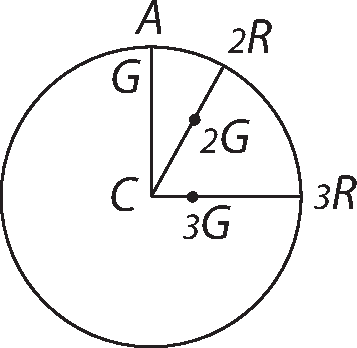
\includegraphics[width=0.21\textwidth]{%
gesamttex/edit_VIII,3/images/LH_35_14_02_002,052_d6_052r.pdf%
}} 
\vspace{0.5em}
\centerline{%
\lbrack\textit{Fig.~6}\rbrack%
}
% \newpage%
\vspace{1.0em}
%
\pstart
%
\edtext{\edlabel{35_14_02_002,052_13a}Si}{%	Trick
\lemma{\hspace*{1,6mm}%
\lbrack\textit{Fig.~6}\rbrack%
}\killnumber%
\Cfootnote{%
Ein gestrichener Entwurf zum Diagramm wird nicht wiedergegeben.%
}}%
%
\edtext{}{% C-Footnote
{\xxref%
{35_14_02_002,052_13a}{35_14_02_002,052_13b}}%
\lemma{Si \lbrack...\rbrack\ linea}%
\Cfootnote{%
\cite{01001}a.a.O., Prop.~LVII, S.~108f.}}
%
%
dum regula \textit{CR} movetur aequabiliter circa \textit{C} et in ea mobile accelerate quaeritur
%
\edtext{linea?\edlabel{35_14_02_002,052_13b}
(\protect\vphantom)+ Ego sic\lbrack:\rbrack}{
\lemma{linea?}
\Bfootnote{(\protect\vphantom)+ 
\textit{(1)} Ego sic: tempore venit regula in 
\textit{(a)} \textit{CR} \textit{(b)} \textit{CN} et eodem tempore venit 
\textit{(aa)} \textit{{\scriptsize 1}G} in \textit{{\scriptsize 2}G}, 
\textit{(bb)} \textbar\ mobile in \textit{G} \textit{streicht Hrsg.} \textbar\ 
\textit{(aaa)} erit 
\textit{(aaaa)} \textit{R{\scriptsize 2}G} 
\textit{(bbbb)} \textit{RG} ut \textit{R}  
\textit{(bbb)} erunt ipsae \textit{RG} ut \textbar\ quadrata  temporum, ergo ut quadra \textit{streicht Hrsg.}\ \textbar\ 
\textit{(2)} Ego sic \textit{L}}}
%
si regula \textit{CR} moveatur circa \textit{C} ex situ \textit{CA}, per situs \textit{CR}, et mobile in ea accelerato uniformiter motu tendat ab \textit{R} versus \textit{C}, et spatium percursum 
%
\edtext{sit \textit{RG}, erunt}{
\lemma{sit \textit{RG},}
\Bfootnote{\textit{(1)} di \textit{(2)} \textbar\ erit \textit{streicht Hrsg.} \textbar\ \textit{R} \textit{(3)} erunt \textit{L}}}
%
\textit{RG} ut quadrata temporum ergo quadrata ipsorum \textit{AR}. 
+\protect\vphantom()
%
\edtext{%
Fuit quidam, qui putavit cognosci posse an navis velocissime sed aequabiliter moveatur an quiescat, idque intra 
%
navem dimittendo
%
\edlabel{35_14_02_002,052_3a}%
\edtext{}{{\xxref{35_14_02_002,052_3a}{35_14_02_002,052_3b}}%
\lemma{grave.}%
\Bfootnote{\textit{(1)} Scilicet quoties proportiones impetum gravis \textit{(2)} Corpus durum impetum \textit{L}}}%
grave.}{%
\lemma{Fuit \lbrack...\rbrack\ grave}%
\Cfootnote{%
\cite{01001}a.a.O., Prop.~LVIII, S.~111.%
}}
%
\pend
%
\pstart
%
\edtext{Corpus durum impetum\edlabel{35_14_02_002,052_3b}
%
incidentis 
%
\edtext{duri}{
\lemma{}
\Bfootnote{duri \textit{erg. L}}}
%
non imminuit.}{%
\lemma{Corpus \lbrack...\rbrack\ imminuit}%
\Cfootnote{%
\cite{01001}a.a.O., Prop.~LIX, S.~115.%
}}
%
\pend
\newpage
\count\Bfootins=1000%
\count\Afootins=1200%
\count\Cfootins=1000 
%
\pstart
\edtext{%
Si corpus excipiens 
%
\edtext{\textit{B} quiescens}{
\lemma{}
\Bfootnote{\textit{B} quiescens \textit{erg. L}}}
%
sit minus incurrente \textit{A}, et corpus excipiens 
%
loco suo sit alligatum quasi, ita ut cum difficultate possit amoveri, superare tamen possit \textit{A} hanc difficultatem,
%
semper reflectetur \textit{A}. Idque etiam contingit cum corpora non sunt omnino dura.}{%
\lemma{Si \lbrack...\rbrack\ dura}%
\Cfootnote{%
\cite{01001}a.a.O., Prop.~LXII, S.~118f.%
}}
%
\pend
%
\pstart
%
\edtext{Prop.~63.}{%
\lemma{Prop.~63.}
\Bfootnote{\textit{erg. L}}}
%
\edtext{Si duo corpora
%
\edtext{dura}{
\lemma{dura}
\Bfootnote{\textit{erg. L}}}
%
velocitatibus reciproce proportionalibus concurrant, redibunt quibus venere velocitatibus\lbrack,\rbrack\ utrumque scilicet movetur quasi in immobile incurreret.}{
\lemma{Si \lbrack...\rbrack\ incurreret}
\Cfootnote{
\cite{01001}a.a.O., Prop.~LXIII, S.~120.}} 
%
\pend 
%
\pstart 
%
(\protect\vphantom)+ NB. Revera non possunt fieri corpora perfecte dura, nam corpus impetus 
%
duos contrarios habens, quiesceret et ita 
%
\edtext{esset perditio}{
\lemma{esset}
\Bfootnote{\textit{(1)} actionum \textit{(2)}~perditio \textit{L}}}
%
impetus. Sed revera in illis 
%
\edtext{casibus\lbrack,\rbrack\ transfertur}{%
\lemma{casibus}%
\Bfootnote{%
\textit{(1)} \textbar\ est \textit{streicht Hrsg.}\ \textbar\  in ipso %
\textit{(2)} transfertur %
\textit{L}%
}}
%
in partes. +\protect\vphantom() %
\pend
%
\pstart
%
%
\hspace{1mm}\hspace{-1mm}% Trick, weil \edlabel nicht zu \par-Beginn sein darf
\edlabel{35_14_02_002,052_15a}%
\edtext{}{% C-Footnote
{\xxref%
{35_14_02_002,052_15a}{35_14_02_002,052_15b}}%
\lemma{Vera \lbrack...\rbrack\  percussione}%
\Cfootnote{%
\cite{01001}a.a.O., Prop.~LXVII, S.~131f.}}%
Vera Borello\protect\index{Namensregister}{\textso{Borelli} (Borellus), Giovanni Alfonso 1608\textendash1679} 
%
(ad prop.~67)
%
extinctionis motus causa, cum duo sint contrarii impetus sine 
%
\edtext{percussione;\edlabel{35_14_02_002,052_15b} (\protect\vphantom)+ sed}{
\lemma{percussione;}
\Bfootnote{\textit{(1)} ut cum navis \textit{(2)} (\protect\vphantom)+ sed \textit{L}}}
%
revera casus non est dabilis in 
%
\edtext{natura \lbrack+\protect\vphantom()\rbrack\ (\protect\vphantom)+ ut si}{
\lemma{natura}
\Bfootnote{%
\textit{(1)} +\protect\vphantom() \textbar\ rigore, ut \textit{streicht Hrsg.} \textbar\ cum a gravitate contrarius imprimitur impetus \textit{(a)} ascens \textit{(b)} descensus impetui ascensus et poneretur \textit{(aa)} gravitationis celeritatem in \textit{(bb)} \textbar\ motum gravitatis \textit{streicht Hrsg.} \textbar\ \textit{(2)} (\protect\vphantom)+ ut si \textit{L}}}
%
poneremus grave descendere motu aequabili (acceleratione a medio consumta) et grave esse tormentum quod 
%
\edtext{explodat pilam}{
\lemma{explodat}
\Bfootnote{\textit{(1)} grave \textit{(2)} pilam \textit{L}}}
%
sursum eique det eandem praecise 
%
\edtext{velocitatem ascensus}{
\lemma{velocitatem}
\Bfootnote{\textit{(1)} quam habet de \textit{(2)} ascensus \textit{L}}}
%
qui est descensus, revera quiescet pila suspensa in aere, deserto tormento. +\protect\vphantom() 
%
\edtext{\textit{Impetus debilitari potest in instanti ob sui} 
%
divisionem\lbrack,\rbrack\ corpus
%
majus \textit{destrui non potest nisi tempore}. \textit{Suspicare licet, motum} non destrui in natura, sed compensari tantum contrario,}{%
\lemma{\textit{Impetus} \lbrack...\rbrack\ contrario}%
\Cfootnote{%
\cite{01001}a.a.O., Cap.~XVII, S.~132.}}
%
(+ ego puto ne sic quidem posse destrui. +) %
\pend
%
\pstart
\edtext{Virga resiliens extinguit impetum percussivum sed eum restituit.}{%
\lemma{Virga \lbrack...\rbrack\  restituit}%
\Cfootnote{%
\cite{01001}a.a.O., Prop.~LXXII, S.~145f.%
}}
\pend
%
\pstart
%
\edtext{Planum impetus vel velocitatis est 
%
Borello\protect\index{Namensregister}{\textso{Borelli} (Borellus), Giovanni Alfonso 1608\textendash1679} 
%
factum ex ductu velocitatis in tempus (+ potius temporis elementum +)\lbrack,\rbrack\ est 
%
rectangulum in motu aequabili, triangulum in uniformiter accelerato.}{%
\lemma{}%
\Cfootnote{%
\hspace{-2.45mm}Planum \lbrack...\rbrack\ accelerato: \cite{01001}a.a.O., Cap.~XX, S.~150f.}}
%
\edtext{\textit{Corpora se moventia aequabili velocitate nunquam delebili agitantur} 
et \textit{debent in natura corpora admitti} hujusmodi \textit{vivida, praeter inertia}.}{%
\lemma{\textit{Corpora} \lbrack...\rbrack\ \textit{inertia}}%
\Cfootnote{%
\cite{01001}a.a.O., Cap.~XXI, S.~160.%
}}
\pend
%\newpage
\pstart
%
\edtext{\textit{Machina intra navem quiescentem resiliens} non potest propellere navem \textit{licet percutiat} anterius \textit{tabulatum.}}{%
\lemma{\textit{Machina} \lbrack...\rbrack\ \textit{tabulatum}}%
\Cfootnote{%
\cite{01001}a.a.O., Prop.~LXXXII, S.~166.%
}}
%
\pend
\newpage
\count\Bfootins=1100%
\count\Afootins=1200%
\count\Cfootins=1100 
%
%\vspace{1.0em} %%%%%%%%% Diagramm 7
\centerline{%
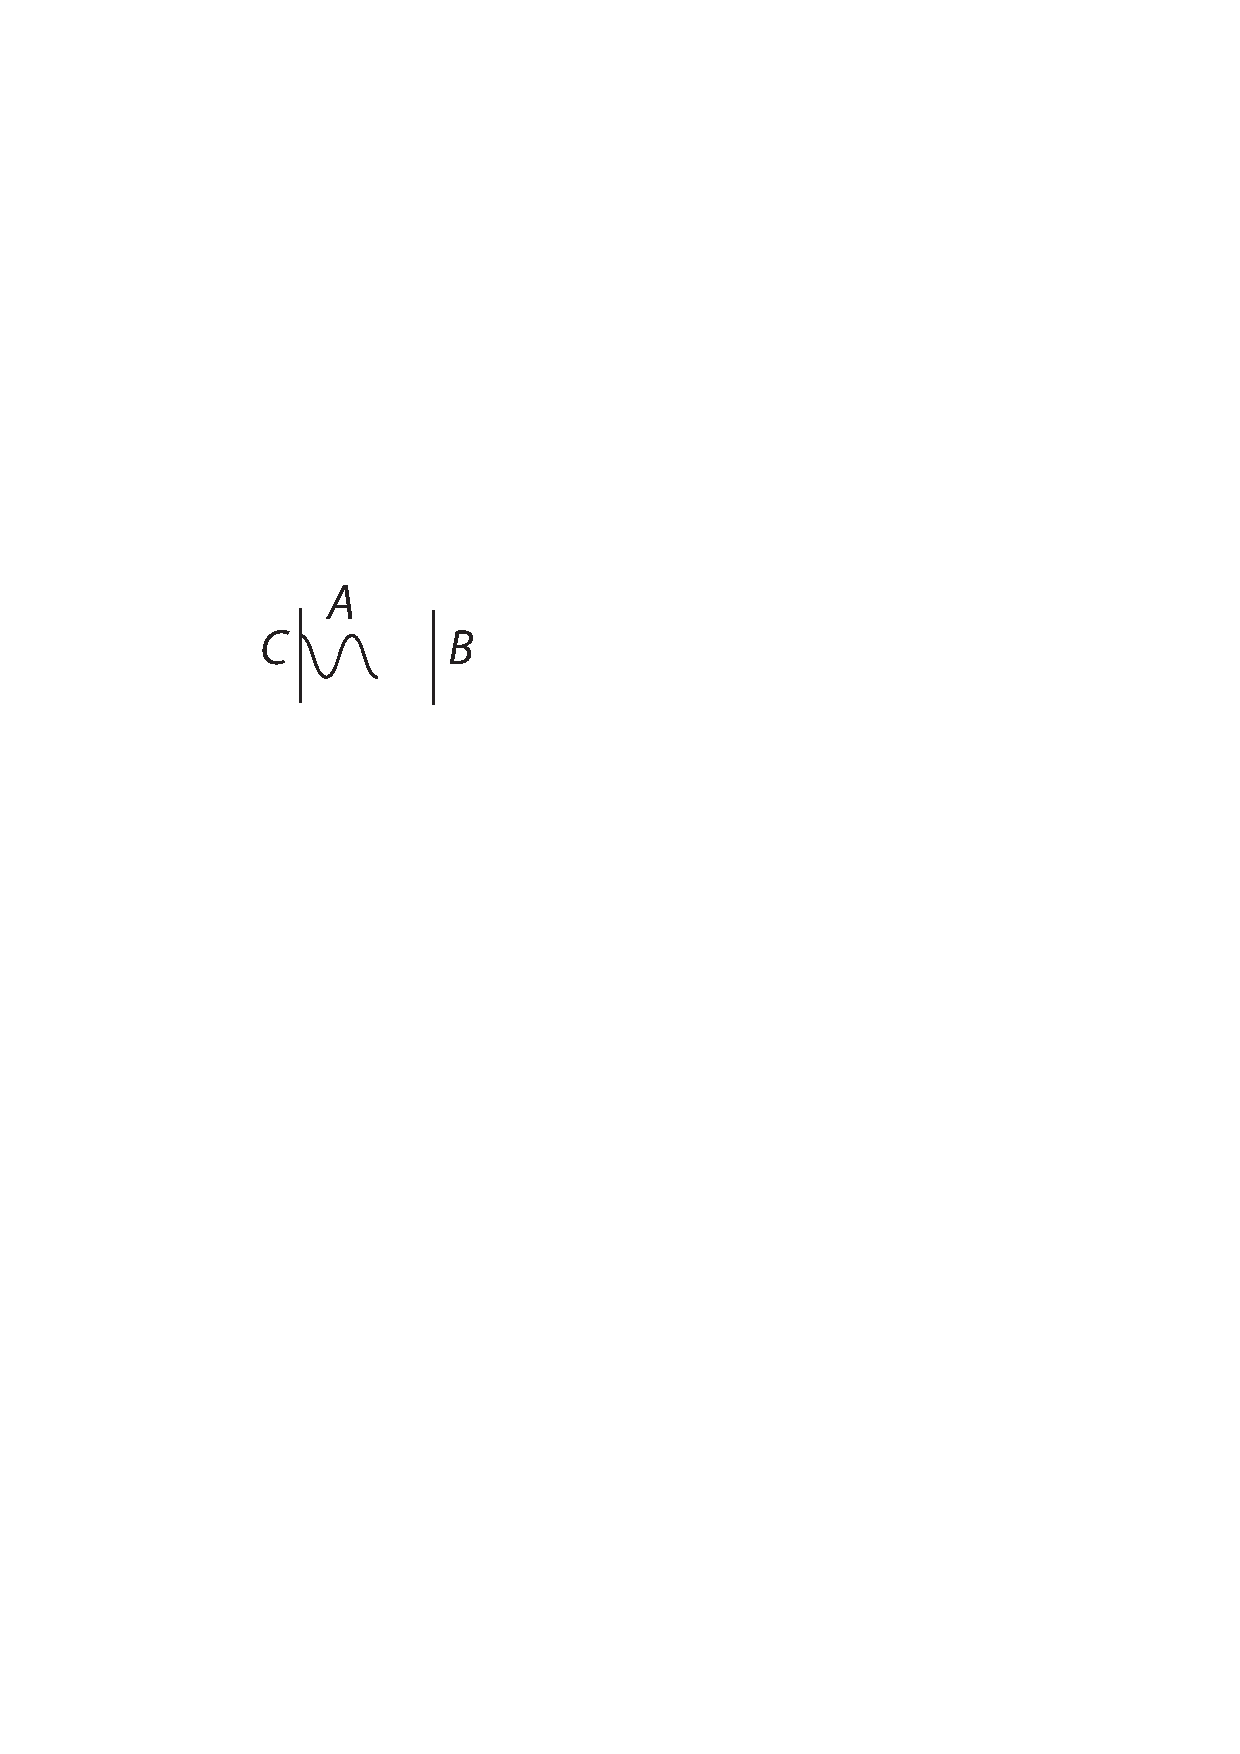
\includegraphics[width=0.125\textwidth]{%
gesamttex/edit_VIII,3/images/LH_35_14_02_002,052_d7_052r.pdf%
}} 
\vspace{0.4em}
\centerline{%
\lbrack\textit{Fig.~7}\rbrack%
}
% \newpage%
\vspace{1.0em}
%
\pstart
%
\edtext{Ut si lamina \textit{A} pressa liberetur et percutiat \textit{B} non promovebit navem, quia quantum \textit{B} impellit in unam partem tantum \textit{C} in contrariam.}{%
\lemma{}%
\Afootnote{%
\textit{Am Rand:} NB}}
%
\pend
%
\pstart 
\lbrack52~v\textsuperscript{o}\rbrack\ 
%
\edtext{Clavus malleo infigi potest \textit{tum a vi compressiva} 
%
\textit{ponderis ingentis}, tum \textit{ab ictu alicujus mallei, et in hac actione comparari debent}
%
\edtext{\textit{inter se vi}\lbrack\textit{s}\rbrack\ \textit{clavum comprimens}}{
\lemma{\textit{inter se}}
\Bfootnote{\textit{(1)} \textit{vis illa} \textit{(2)} \textbar\ vires \textit{ändert Hrsg.}\ \textbar\ %
 \textit{(a)} clavum infig \textit{(b)} \textit{clavum comprimens} \textit{L}}}
%
\textit{et resistentia duri} cui \textit{est} infigendus.}{%
\lemma{Clavus \lbrack...\rbrack\ infigendus}%
\Cfootnote{%
\cite{01001}a.a.O., Cap.~XXVII, S.~192f.}}
%
\edtext{\textit{Secundus} mallei \textit{ictus profundius clavum infigit,} 
%
\edtext{sed ad clavum infigendum}{
\lemma{sed ad}
\Bfootnote{\textit{(1)} imprimendum \textit{(2)} clavum infigendum \textit{L}}}
%
ad eandem altitudinem opus est gravitate 
%
\edtext{plus quam}{
\lemma{plus quam}
\Bfootnote{\textit{erg. L}}}
%
dupla prioris. Ergo ictus mallei plus quam libris 200.\ aequatur et quia tertio ictu rursus altius figitur clavus 
%
quam possit novo pondere 300 librarum infigi, ergo aequatur plus quam 300 libris, et sic in infinitum\lbrack,\rbrack\ ergo vis
%
\edtext{mallei percutientis infinita videtur.}{			
\lemma{mallei}
\Bfootnote{\textbar\ percutientis \textit{erg.} \textbar\ \textit{(1)} \textbar\ est \textit{streicht Hrsg.} \textbar\ infinita \textit{(2)} infinita videtur. \textit{L}}}%
}{%
\lemma{\textit{Secundus} \lbrack...\rbrack\ videtur}%
\Cfootnote{%
\cite{01001}a.a.O., S.~195f.}}
%
Sed revera hoc non 
%
\edtext{probat, nam}{
\lemma{probat,}
\Bfootnote{\textit{(1)} \textbar\ perinde est \textit{streicht Hrsg.} \textbar\ enim ac si \textit{(a)} infiniti  \textbar\ essent \textit{streicht Hrsg.} \textbar\ \textit{(b)} mallei repetit \textit{(2)} nam \textit{L}}}
%
percussiones repetitae sunt ut percussiones mallei toties majoris in infinitum. Et considerandum in gravitate aequalem esse 
%
\edtext{vim gravis}{
\lemma{vim}
\Bfootnote{\textit{(1)} gravitatis \textit{(2)} gravis \textit{L}}}
%
et resistentis, cum malleus ultra infigi non potest. At in vi percussionis non ideo 
%
\edtext{cessat infixio}{
\lemma{cessat}
\Bfootnote{\textit{(1)} operatio \textit{(2)} actio \textit{(3)} infixio \textit{L}}}, 
%
sed quia cessat operatio 
%
%
\edlabel{35_14_02_002,052_10a}%
\edtext{}{% B-Footnote
{\xxref%
{35_14_02_002,052_10a}{35_14_02_002,052_10b}}%
\lemma{percutientis}
\Bfootnote{\textit{(1)} (\protect\vphantom)+ hoc nihil est in grave decidente \textit{(2)} paulatim destructi. \textit{(a)} Objectio con \textit{(b)} Objectio contra infinitam \textit{(c)} Probat melius vim percussionis infinitam elevando \textit{(aa)} , quia \textit{(bb)} dum \textit{L}}}%
%
percutientis paulatim destructi. %
\pend
%
\pstart
Probat melius vim percussionis infinitam elevando, 
%
\edtext{dum%
\edlabel{35_14_02_002,052_10b}
%
fingit corpus \textit{A} et \textit{B} cadere in opposita librae brachia ubi vis erit aequalis si sint velocitates reciproce proportionales, 
%
ergo si \textit{B} habet velocitatem nullam utique attolletur.}{%
\lemma{dum \lbrack...\rbrack\ attolletur}%
\Cfootnote{%
\cite{01001}a.a.O., Prop.~XC, S.~203\textendash205.%
}}
%
\pend 
%\newpage
\count\Bfootins=1100%
\count\Afootins=1200%
\count\Cfootins=1100 
%
\pstart 
%
\edtext{Objicitur facilius nos tolerare ictum lapilli, quam pondus vasti corporis, sed vis percussionis non est perseverans 
%
sed \textit{destruitur mollitie partium animalis, pondus in progressu compressionis semper aequilibrari debet}.}{%
\lemma{Objicitur \lbrack...\rbrack\ \textit{debet}}%
\Cfootnote{%
\cite{01001}a.a.O., S.~207\textendash209.%
}}
%
%
\edtext{Deinde revera \textit{saxum ingens sine aliquo impetu applicari animali} non potest.}{%
\lemma{Deinde \lbrack...\rbrack\ potest}%
\Cfootnote{%
\cite{01001}a.a.O., S.~210.}}
%
(\protect\vphantom)+ Imo sic satis potest ponendo scindi chordam tenentem. +\protect\vphantom()
%
(\protect\vphantom)+ Omne elastrum perfectum utcunque tensum pondere novo simpliciter imposito sine 
%
impetu nonnihil adhuc deprimetur in tantum ut vis quae est 
%
\edtext{ponderis per}{%
\lemma{ponderis}%
\Bfootnote{%
\textit{(1)} in %
\textit{(2)} per %
\textit{L}%
}}
%
talem altitudinem descendentis sit tali 
%
tensioni elastri aequalis. +\protect\vphantom() 
%
\edtext{Corpora quae rigida censentur sunt congeries machinarum flexibilium et se restituentium.}{%
\lemma{Corpora \lbrack...\rbrack\  restituentium}%
\Cfootnote{%
\cite{01001}a.a.O., Prop.~XCVII, S.~218.}}
%
\pend 
%					
\vspace{0.8em} %%%%%%%%% Diagramm 8
\centerline{%
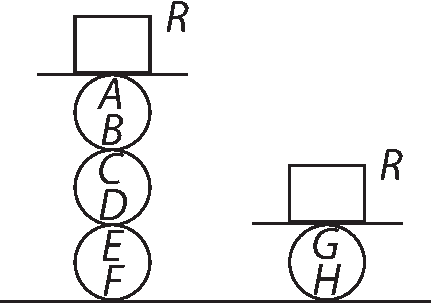
\includegraphics[width=0.275\textwidth]{%
gesamttex/edit_VIII,3/images/LH_35_14_02_002,052_d8_052v.pdf%
}} 
\vspace{0.3em}
\centerline{%
\lbrack\textit{Fig.~8}\rbrack%
}
% \newpage%
\vspace{0.9em}
%
%
\pstart
%
\edtext{\edlabel{35_14_02_002,052_16a}}{% Trick für Figur
\lemma{\hspace{1.7mm}\lbrack\textit{Fig.~8}\rbrack}\killnumber\Cfootnote{Tlw.\ Übernahme der Vorlage: \cite{01001}a.a.O., Tabula quarta, Fig.~82.}}%
\edtext{}{% C-Footnote
{\xxref%
{35_14_02_002,052_16a}{35_14_02_002,052_16b}}%
\lemma{Si \lbrack...\rbrack\ armillarum}%
\Cfootnote{%
\cite{01001}a.a.O., Prop.~C, S.~222f.%
}}%
Si plures armillae ferreae aequales inter se et sibi superpositae 
%
premantur a pondere \textit{R}, tantum comprimetur quaelibet 
%
earum quantum similis et aequalis ipsis \textit{GH}, si sola a pondere eodem \textit{R} premeretur\lbrack,\rbrack\ sed descensus ipsius \textit{R} 
%
\edtext{erit major illic in ratione}{
\lemma{erit}
\Bfootnote{\textit{(1)} triplo \textit{(2)} major \textit{(a)} in tribus \textit{(b)} illic \textit{(aa)} quam hic \textit{(bb)} in ratione \textit{L}}}
%
armillarum.%
\edlabel{35_14_02_002,052_16b}
\pend
%
\pstart
\edtext{(\protect\vphantom)+ Recte nam triplum
%
effectum effecit, ergo triplus quoque descensus. Certe omnes armillae tres aequaliter pressae, 
%
\edtext{alioqui magis}{
\lemma{alioqui}
\Bfootnote{\textit{(1)} una alteram \textit{(2)} mot \textit{(3)} magis \textit{L}}}
%
pressae se liberarent contra}{\lemma{}\Afootnote{\textit{Am Rand}: NB\vspace{-6mm}}} 
%
minus pressas, praeterea ubi satis pressum est \textit{CD}, ut non amplius premi possit, 
%
vim habet plani resistentis sine ulteriore 
%
\edtext{flexione. Ergo}{
\lemma{flexione.}
\Bfootnote{\textit{(1)} Ergo \textit{(2)} Perinde est ac si \textit{AB} esset ipsa \textit{GH} sola su \textit{(3)} Ergo \textit{L}}}
%
\textit{AB} super \textit{CD} est ut \textit{GH} super plano non cedente. \lbrack+\protect\vphantom()\rbrack\
%
\edtext{% C-Fn
\hspace{1mm}\hspace{-1mm}% Trick,
\edtext{Eadem si percutiendo}{%
\lemma{Eadem si}%
\Bfootnote{%
\textit{(1)} quod %
\textit{(2)} percutiendo %
\textit{L}%
}}
%
incideret pondus, et 
%
rursus ab armillis repercuteretur. 
%
Plures itaque armillae corpus repellent altius.}{%
\lemma{Eadem \lbrack...\rbrack\ altius}%
\Cfootnote{%
\cite{01001}a.a.O., Prop.~CI, S.~223\textendash225.}}
\pend
%
\pstart
\edtext{Aer dirumpit aeneas fistulas et tamen non tangitur nisi ab extremis machinulis, quae subtiliores omni filo.}{%
\lemma{Aer \lbrack...\rbrack\ filo}%
\Cfootnote{%
\cite{01001}a.a.O., Prop.~CII, S.~226f.}}
%
\pend 
\newpage
%
\pstart 
\edtext{Primus serenissimus princeps Leopoldus ab Etruria\protect\index{Namensregister}{\textso{Medici}, Leopoldo de' (Leopoldus) 1617\textendash1675}
%
\edtext{observavit si phiala vitrea}{
\lemma{observavit}
\Bfootnote{\textit{(1)} phialam \textit{(2)} si phiala \textit{(a)} vitrea \textit{(aa)} con \textit{(bb)} immergatur in aquam subito \textit{(aaa)} situm \textit{(bbb)} so \textit{(ccc)} contrahere \textit{(b)} vitrea \textit{L}}}
%
aqua plena immergatur in aquam calidam, tunc aquam in phiala descendere\lbrack,\rbrack\ si in nivem ascendere.
%
\edtext{Ratio quod calor}{%
\lemma{Ratio}%
\Bfootnote{%
\textit{(1)} quod  comp %
\textit{(2)} quod %
\textit{(a)} aqu %
\textit{(b)} calor~\textit{L}%
}}
%
igniculis quibusdam 
%
insertis dilatat poros.}{%
\lemma{Primus \lbrack...\rbrack\ poros}%
\Cfootnote{%
\cite{01001}a.a.O., Prop.~CV, S.~236f.}} 
%
\edtext{Iidem 
%
\edtext{cunei in annulo}{
\lemma{cunei}
\Bfootnote{\textit{(1)} in ampliore superficie minore vi in \textit{(2)} in annulo \textit{L}}}
%
curvato a parte exteriore poros magis amplos inveniunt, et ideo minorem vim exercent.
Sic corpora fluida minore vi excurrunt per canales dilatatos.}{%
\lemma{Iidem \lbrack...\rbrack\ dilatatos}%
\Cfootnote{%
a.a.O., S.~238.%
}}
%
\pend
%
\pstart
%
\edtext{\textit{Vis compressiva ambientis fluidi porositates armillae ampliatas} rursus 
%
\textit{constringere}, et sic restitutionem facere \textit{potest}.}{%
\lemma{\textit{Vis} \lbrack...\rbrack\ \textit{potest}}%
\Cfootnote{%
\cite{01001}a.a.O., Prop.~CVII, S.~241 mit Auslassungen.%
}}
%
\edtext{Idem facere possent particulae igneae motae.}{%
\lemma{Idem \lbrack...\rbrack\ motae}%
\Cfootnote{%
\cite{01001}a.a.O., Prop.~CVIII, S.~242.%
}}
%
\edtext{%
\hspace{1mm}\hspace{-1mm}% Trick
\edtext{Quia motus}{
\lemma{Quia}
\Bfootnote{\textit{(1)} vis \textit{(2)} motus \textit{L}}}
%
vehementior producere potest motum languidum, vicissim languidus potest producere vehementiorem.}{%
\lemma{Quia \lbrack...\rbrack\ vehementiorem}%
\Cfootnote{%
\cite{01001}a.a.O., Cap.~XXXII, S.~245.}}
%
(\protect\vphantom)+ Hoc ego sic\lbrack:\rbrack\ 
%
\edtext{dum magnum a parvo impulsum,}{
\lemma{dum}
\Bfootnote{\textit{(1)} per magnum \textit{(2)} magnum a parvo \textit{(a)} in quiescente \textit{(b)} impulsum, \textit{L}}}
%
quod post quiescit, rediens iterum quiescet et dabit parvo motum 
%
%
\edlabel{35_14_02_002,052_17a}%
\edtext{}{% B-Footnote
{\xxref%
{35_14_02_002,052_17a}{35_14_02_002,052_17b}}%
\lemma{celeriorem. +\protect\vphantom()}
\Bfootnote{\textit{(1)} Languidissimus tremor rep 
\textit{(2)} \textbar\ Autor \textit{streicht Hrsg.}\ \textbar\ intelligit per repetitionem percussionis, ut si pendulum \textbar\ parvum \textit{erg.} \textbar\ in corpus incidat, et reflectatur et deinde rursus in ipsum incidat \textit{(3)} . Languidissimus \textit{L}}}%
celeriorem. +\protect\vphantom() 
%
\edtext{\textit{Languidissimus}%
\edlabel{35_14_02_002,052_17b}
%
\textit{tremor tubae vel tympani tremorem} integro templo dat continuatione.}{%
\lemma{}%
\Cfootnote{%
\hspace{-2.75mm}\textit{Languidissimus} \lbrack...\rbrack\ continuatione: \cite{01001}a.a.O., Prop.~CXI, S.~247.}}
%%
\pend
%
\pstart
%
\edtext{Cum Aethna\protect\index{Sachverzeichnis}{Aetna} eruptionem faceret
%
eram \protect\index{Ortsregister}{Taormina}Tauromenii 
%
quod distat 30 miliaribus. Eruptione Aetnae\protect\index{Sachverzeichnis}{Aetna} tremebant omnia 
%
\protect\index{Ortsregister}{Taormina}Tauromenii aedificia sed illa magis quae conspectum habebant 
%
voraginis seu Aetnae\protect\index{Sachverzeichnis}{Aetna}\lbrack,\rbrack\ reliqua lentius multo, 
%
non enim erat a solo, sed 
%
\edtext{\lbrack\textit{a tremore}\rbrack}{%
\lemma{}%
\Bfootnote{%
\textit{a tremore} %
\textit{erg.\ Hrsg.\ nach Vorlage}%
}}
%
\textit{aeris incussi}
%
\edlabel{35_14_02_002,052_11a}%
\edtext{}{% B-Footnote
{\xxref%
{35_14_02_002,052_11a}{35_14_02_002,052_11b}}%
\lemma{\textit{parietibus}.}%
\Bfootnote{%
\textit{(1)} \textit{Sagitta}
\textit{(2)}~Borell.}}%
\textit{parietibus}.}{%
\lemma{Cum \lbrack...\rbrack\ \textit{parietibus}}%
\Cfootnote{%
\cite{01001}a.a.O., S.~248f.}}
%%
\pend
%
\pstart
Borell.\protect\index{Namensregister}{\textso{Borelli} (Borellus), Giovanni Alfonso 1608\textendash1679}%
\edlabel{35_14_02_002,052_11b} 
%
\edtext{prop.~\lbrack114.\rbrack}{
\lemma{}
\Bfootnote{prop.~14. \textit{L ändert Hrsg.}}} 
%
\edtext{\textit{Sagitta vel pila lignea} 
%
\edtext{sursum projecta}{
\lemma{}
\Bfootnote{sursum projecta \textit{erg. L}}}
%
\textit{percurrit} ferme \textit{spatium duplum ascendendo, quam} percurrit
%
\textit{descendendo},
%
quod deberet esse idem, et impetus quaesitus descensu multo minor est quam fuit ab initio.}{%
\lemma{\textit{Sagitta} \lbrack...\rbrack\ initio}%
\Cfootnote{%
\cite{01001}a.a.O., Prop.~CXIV, S.~257.}}
%
\pend 
%
\pstart 
Prop.~118.
%
\edtext{\textit{Si mobile duabus inaequalibus velocitatibus percutiat idem quiescens amovibile, erunt velocitat}\textlangle\textit{es}\textrangle\ \textit{impressae proportionales} velocitatibus percutientis.}{%
\lemma{\textit{Si} \lbrack...\rbrack\ percutientis}%
\Cfootnote{%
\cite{01001}a.a.O., Prop.~CXVIII, S.~264.}}
%						
\edtext{Problema, quas velocitates habe\textlangle re debeat\textrangle\ ut diversis corporibus 
%
aequales velocitates imprimat.}{%
\lemma{Problema \lbrack...\rbrack\ imprimat}%
\Cfootnote{%
\cite{01001}a.a.O., Prop.~CXIX, S.~265.}}
%
Percussa \textit{B} et \textit{C}, debet esse 
%
\edtext{velocitas pro}{
\lemma{velocitas}
\Bfootnote{\textit{(1)} major \textit{(2)} pro \textit{L}}}
%
percutiendo \textit{B} ad eam pro \textit{C} ut $A+B$ ad $A+C$. %
\pend
%
\pstart
%
\edtext{\textit{Si idem corpus aequalibus velocitatibus} percutiat \textit{inaequalia}\lbrack,\rbrack\ 
%
\textit{summae percutientis et cujuslibet percussorum} sunt \textit{reciproce proportionales impressis velocitatibus.}}{%
\lemma{\textit{Si} \lbrack...\rbrack\ \textit{velocitatibus}}%
\Cfootnote{%
\cite{01001}a.a.O., Prop.~CXXII, S.~268.}}
%
\pend
%
\pstart
%
\edtext{\textit{Si duo inaequalia} (+ intellige semper dura corpora +) \textit{velocitatibus aequalibus percusserint idem corpus} 
%
\edtext{\textit{(durum)}\lbrack,\rbrack\ \textit{impressae velocitates}}{
\lemma{\textit{(durum)}}
\Bfootnote{\textit{(1)} \textit{perpendiculari} \textit{(2)} \textit{impressae velocitates}~\textit{L}}}
%
erunt in ratione composita 
%
\textit{percutientium corporum et ratione reciproca eorundem una cum corpore percusso}.}{%
\lemma{\textit{Si} \lbrack...\rbrack\ \textit{percusso}}%
\Cfootnote{%
\cite{01001}a.a.O., Prop.~CXXIII, S.~269.}}
\pend
%
\pstart
%
\edtext{\textit{Dato corpore gravi cujus gradus} 
\textit{impetus augeantur juxta seriem numerorum ab unitate incipientium}\lbrack,\rbrack\ 
\textit{corpora percussa} ut accipiant \textit{aequales impetus} crescere 
\textit{debent arithmetica prop.} et \textit{excessus erit aequalis} summae 
percutientis \textit{cum minimo corpore}\lbrack,\rbrack}{%
\lemma{\textit{Dato} \lbrack...\rbrack\ \textit{corpore}}%
\Cfootnote{%
\cite{01001}a.a.O., Prop.~CXXV, S.~272.}} 
%
\edtext{quod impetu}{
\lemma{quod}
\Bfootnote{\textit{(1)} gravi \textit{(2)} impetu \textit{L}}}
%
percutientis aucto et impressa velocitate aequali, crescunt corpora percussa. %
\pend
%
\pstart
%
\edtext{Mersennus\protect\index{Namensregister}{\textso{Mersenne} (Mersennus), Marin 1588\textendash1648} metiendo quantum corpora labentia attollant pondera 
deceptus est a longioribus funiculis impetum absorbentibus distractione.}{%
\lemma{Mersennus \lbrack...\rbrack\ distractione}%
\Cfootnote{%
\cite{01001}a.a.O., Prop.~CXXXII, S.~285f.\hspace{-2mm}}}
%
%\edtext{Mersennus\protect\index{Namensregister}{\textso{Mersenne} (Mersennus), Marin 1588\textendash1648}}{\lemma{Mersennus}\Cfootnote{\textsc{M. Mersenne}, 
%Reflexiones Physico\textendash Mathematicae, cap. VIII, S. 108\textendash110, in: Novae Observationes Physico\textendash Mathematicae, Paris 1647.}}
%
\pend 
%
\pstart 
\edtext{Falsum est experientia probante \textit{impetus} percussivos aequari \textit{resistentiis corporum gravium eandem proportionem habentium quam} habent \textit{impetus}.}{%
\lemma{Falsum \lbrack...\rbrack\ \textit{impetus}}%
\Cfootnote{%
a.a.O., S.~289.\hspace{-2mm}%
}}
%%
\pend
%
\pstart
%
\edtext{\textit{Eadem securicula eadem velocitate efficit} 
%
\textit{altiorem scissuram in cera quam in plumbo, at adhibitis ponderibus supra securim} 
%
\edtext{\textit{ut efficiant scissuras prioribus aequales}}{
\lemma{\textit{ut efficiant scissuras prioribus aequales}}
\Bfootnote{\textit{erg. L}}}
%
\textit{necesse est ut minor scissura plumbi} 
%
\edtext{\lbrack\textit{efficiatur}\rbrack}{%
\lemma{exhibeatur}%
\Bfootnote{%
\textit{L ändert Hrsg. nach Vorlage}%
}}
%
\textit{a majori pondere incumbente, et major scissura cerae efficiatur a} 
%
\edtext{\lbrack\textit{minori}\rbrack}{
\lemma{}
\Bfootnote{majori \textit{L ändert Hrsg. nach Vorlage}}} 
%
\textit{pondere}.}
%
{\lemma{\textit{Eadem} \lbrack...\rbrack\ \textit{pondere}}
\Cfootnote{%
\cite{01001}a.a.O., Prop.~CXXXVI, S.~298.}} 
%
\pend
\count\Bfootins=1200%
\count\Afootins=1200%
\count\Cfootins=1200 
%
%
%
%